
%   Template - Institute of Control Systems, TUHH

%#############################################################################
%     R E A D      M E     F I R S T  !
%#############################################################################
% For setting up a latex enviroment, please follow: https://www.latexbuch.de/latex-windows-installieren/
% In Texmaker you can setup fast compile with these arguments: lualatex -interaction=nonstopmode %.tex|biber %|lualatex -interaction=nonstopmode %.tex|"C:/Program Files/Adobe/Reader 11.0/Reader/AcroRd32.exe" %.pdf
% Possible compilation processes:
% Luatex -> biber -> Luatex 
% For texstudio: lualatex.exe -synctex=1 -interaction=nonstopmode --enable-write18 -interaction=nonstopmode %.tex or pdflatex.exe -synctex=1 -interaction=nonstopmode -shell-escape --enable-write18 -interaction=nonstopmode %.tex
% enables the compiler to use tikz externalize as well
% Toolchain is than: PDFLatex: txs:///pdflatex | txs:///biber | txs:///pdflatex | txs:///view-pdf-internal --embedded
%					  LuaLatex: txs:///lualatex | txs:///biber | txs:///lualatex | txs:///view-pdf-internal --embedded
% VS-Code + LatexWorkshop: Config-File in header/VS_Settings.json
%#############################################################################

%%################ Language settings #########################################

\def\isenglish{true}	% change to false for German language

%%################ DRAFT settings ############################################
\def\isDraft{false}		% Change to false for final project description

 %%################ Document settings #########################################
\def\curdir{}
\documentclass[compress,aspectratio=169]{beamer}

\mode<presentation>
{
  \usetheme{RT}
  \setbeamercovered{transparent}
  \usecolortheme{RT}
}

\setbeamertemplate{navigation symbols}{}
\setbeamertemplate{footline}[frame number]{}


\usepackage{ifthen}
\ifthenelse{\equal{\isenglish}{true}}{
	%%% English
	\usepackage[german, ngerman, english]{babel}
	\selectlanguage{english}
}{
	%%% German
	\usepackage[english, german, ngerman]{babel}
	\selectlanguage{german}
}

\usepackage{lmodern}
\usepackage{csquotes}
\usepackage{microtype}
\ifluatex
	\usepackage{fontspec}
\else
	\usepackage[utf8]{inputenc}
\fi

%% Allow usage of the part command to create different navigations parts 
\usepackage{xpatch}
\makeatletter
\xpatchcmd{\beamer@part}{\Hy@writebookmark{\the\c@section}{#1}{Outline\the\c@part}{1}{toc}}{}{}{}
\makeatother

\usepackage{appendixnumberbeamer}

\makeatletter
\AtBeginPart{%
  \beamer@tocsectionnumber=0\relax
  \setcounter{section}{0}
%   \frame{\partpage}%
}
\makeatother


 %%######## GRAPHICS Options
\graphicspath{{figures/}}				% Define the path to the figures

\usepackage{ifpdf}

 % Other figures (e.g., MATLAB  EPS or PDF figures)
\newcommand{\afig}[2]{\includegraphics[scale=#1]{#2}}

 % figures defined in TeX files
\newcommand{\tfig}[2]{\scalebox{#1}{\input{"#2.tex"}}}


\usepackage{tikz}

\usetikzlibrary{%
  arrows,%
  arrows.meta,
  shapes.misc,% wg. rounded rectangle
  shapes.arrows,
  shapes.misc,
  calc,
  plotmarks,
  chains,%
  matrix,%
  positioning,% wg. " of "
  scopes,%
  decorations.pathmorphing,% /pgf/decoration/random steps | erste Graphik
  decorations.markings,
  shadows%
}
\usetikzlibrary{external}
\tikzexternalize[prefix=figures/] % activate!
\usepackage{pgfplots}
\pgfplotsset{compat=newest}

\newlength{\figw}
\setlength{\figw}{0.8\textwidth}
\newlength{\figh}
\setlength{\figh}{0.4\textwidth}

\newcommand{\tikzfig}[2]{
  \tikzsetnextfilename{#2}%
  \scalebox{#1}{
    \input{"figures/#2.tex"}}
}

 %%######## Logos only on Title page

\titlegraphic{
	% \vspace{1cm}
	\begin{minipage}{0.5\textwidth}
		\begin{flushleft} \large
			\ifthenelse{\equal{\isenglish}{true}}
			{
\includegraphics[height=1.5cm]{admin/Logo_TUHH_en}}
			{
\includegraphics[height=1.5cm]{admin/Logo_TUHH_de}}
		\end{flushleft}
	\end{minipage}
	\hfill
	\begin{minipage}{0.4\textwidth}
		\begin{flushright} \large
			
\includegraphics[height=1.5cm]{admin/Logo_ICS_4c} % Supervisor's Name
		\end{flushright}
	\end{minipage}\\[0.4cm]
}

 %%######## Other FUNCTIONS

 % Some color definitions
\setbeamercolor{greenhead}{fg=white,bg=green!80!black}%
\setbeamercolor{greenbody}{fg=black,bg=green!50!white}%

\setbeamercolor{redhead}{fg=white,bg=red!80!black}%
\setbeamercolor{redbody}{fg=black,bg=red!50!white}%


\usepackage{epstopdf}

\usepackage[style=ieee,backend=biber]{biblatex} %% bibliography
% \usepackage{biblatex}

\usepackage{multicol}
\usepackage{subfig}
\usepackage{graphicx}
\usepackage{svg}
\usepackage{tikz}
\usetikzlibrary{shapes, arrows, positioning}
\addbibresource{ics.bib}





 %%#######################################################
 %%################## Thesis Data ######################

% Student Entry No.               1

\def\titlenameEN{Data Driven Model Predictive Control using Gaussian Processes}

\def\titlenameDE{Datengetriebene modelprädiktive Regelung mit Gaußschen Prozessen}

\def\authorfirstname{Harshith}
\def\authorfamilyname{Gowda}

% f: female
% m: male 
\def\gender{m}

\def\studentid{565699}

\def\studycourse{MEC}

% p: project work
% b: bachelor thesis
% m: master's thesis
\def\thesistype{p}

\def\thesisnumber{\MakeUppercase{\thesistype} --- 2 --- 2024}

\def\supervisornameI {Jannis Lübsen, M.Sc.}


\def\supervisornameII {}


\def\examinernameI {Prof. Dr.-Ing Annika Eichler}


\def\examinernameII {Jannis Lübsen, M.Sc.}

% If written externally, like in a Company or at another university, note this university here
% A supervisor of the company can be put as supervisor
\def\ExternalCompany {}

% Shows if the thesis is under NDA, only displayed when ExternalCompany is set
% false: no NDA
% true: NDA
\def\HasNDA {false}
% Set date until the NDA is agreed, normally duedate + 3 years
\def\NDAdueDate {}


\def\startdate{06.05.2019}

\def\duedate{18.08.2019}

\def\todaydate{14.06.2019}


 % Project description
\def\projectdescription{
	Model predictive control (MPC) has gained more attention in the past years as it is a powerful modern control technique which relies on repeatedly solving an open-loop optimal control problem. In order to obtain high-quality optimal input signals, an accurate prediction model is required, which is often unavailable or difficult to identify. In recent years data-driven control approaches have become more interesting because they use only measured data to control unknown systems without prior model identification. A major issue in data-driven control is the treatment of measurement noise, which in recent publications is treated to be deterministically bounded \cite{Berberich_2021}.  However, this assumption does not generally hold for a real system.
	
	Alternatively, a stochastic model can be used to model the state transition function as in \cite{kamthe2018}. However, there is a lack of theoretical guarantees of proabalistic models, e.g., Gaussian processes.
	
	The goal of this thesis is to implement a probabilistic MPC scheme relying on Gaussian process models to represent the transition function of a nonlinear time-discrete system with noisy measurements. Therefore, a multioutput Gaussian process model consisting of independent subprocesses is considered. A challenge is the definitions of suitable constraints for the optimization procedure, e.g., state constraints, since states are no longer deterministic but stochastically distributed. 
	
	Within the scope of the work, a literature review on Gaussian processes and probabilistic MPC will first be conducted. Then, the method should will be implemented and tested in simulation. If this was successful, the algorithm should be tested on a real plant. Finally, the experimental data will be evaluated and the results obtained will be discussed. 
}

 % Project tasks
\def\tasks{
\begin{packedenumerate}
	\item Literature review
	\item Familiarization with Gaussian processes and MPC 
	\item Implementation of the probabilistic MPC algorithm
	\item Comparison to other (probabilistic) MPC algorithms/implementations
	\item Testing in simulation and, if successful, testing on a real plant
	\item Evaluation and discussion
\end{packedenumerate}
}


 %%##############################  CONTENTS ###################################
\begin{document}

 %% Title page
\thispagestyle{empty}
\pagenumbering{Roman}

\begin{titlepage}

 %%################ general settings ###################
\definecolor{darkBlue}{rgb}{0, 0.255, 0.471} 
\newcommand{\HRule}{\textcolor{darkBlue}{\rule{\textwidth}{0.4mm}}} % Defines a new command for the horizontal lines, change thickness here
\center % Center everything on the page

% thesis type
\ifthenelse{\equal{\isenglish}{true}}{
	\ifthenelse{\equal{\thesistype}{m}}{
		\def\thesisname{Master's thesis}}
	{\ifthenelse{\equal{\thesistype}{b}}{
		\def\thesisname{Bachelor thesis}}
	{\ifthenelse{\equal{\thesistype}{p}}{
		\def\thesisname{Project work}}{
		\def\thesisname{\thesistype}
	}}}
}
{
	\ifthenelse{\equal{\thesistype}{m}}{
		\def\thesisname{Masterarbeit}}
	{\ifthenelse{\equal{\thesistype}{b}}{
		\def\thesisname{Bachelorarbeit}}
	{\ifthenelse{\equal{\thesistype}{p}}{
		\def\thesisname{Projektarbeit}}{
		\def\thesisname{\thesistype}
	}}}
}

 %%################ logo section ###################
\HRule \\[0.4cm]
\begin{minipage}{0.5\textwidth}
\begin{flushleft} \large
	\ifthenelse{\equal{\isenglish}{true}}
	{
\includegraphics[height=3cm]{admin/Logo_TUHH_en}}
	{
\includegraphics[height=3cm]{admin/Logo_TUHH_de}}
\end{flushleft}
\end{minipage}
\hfill
\begin{minipage}{0.4\textwidth}
\begin{flushright} \large

\includegraphics[height=3cm]{admin/Logo_ICS_4c} % Supervisor's Name
\end{flushright}
\end{minipage}\\[0.4cm]

\HRule \\[3cm]
 {\large \textsc{\thesisname}}\\[1cm]
{\fontsize{32}{32}\selectfont
\ifthenelse{\equal{\isenglish}{true}}{\titlenameEN}{\titlenameDE}\par
}

\vfill

 %%################ author and date section ###################

\begin{minipage}[b]{0.6\textwidth}
\begin{flushleft} \large
\ifthenelse{\equal{\isenglish}{true}}{\emph{Author:}}{\emph{Autor:}}\\
\authorfirstname\, \authorfamilyname \\[1cm] % Your name
%\ifthenelse{\equal{\isenglish}{true}}{\emph{Supervisors:}}{\emph{Betreuer:}} \\
%\supervisorname
%\ifthenelse{\equal{\isenglish}{true}}{\emph{Examiners:}}{\emph{Gutachter:}} \\
%\examinername

%%################ Supervison section ###################
\begin{tabbing}
\textbf{\ifthenelse{\equal{\isenglish}{true}}{Supervisor:}{Betreuer:\hspace{0.4cm}}} \= \phantom{1.} \= \supervisornameI \\ \> \phantom{2.} \> \supervisornameII \\
\textbf{\ifthenelse{\equal{\isenglish}{true}}{Examiner:}{Prüfer:}} \> \ifthenelse{\equal{\examinernameII}{}}{}{1.}  \> \examinernameI \\
\ifthenelse{\equal{\examinernameII}{}}{}{\> 2. \> \examinernameII}
\end{tabbing}

\end{flushleft}
\end{minipage}
\hfill
\begin{minipage}{0.3\textwidth}
\begin{flushright}
{\large \today} % Date, change the \today to a set date if you want to be precise
\end{flushright}
\end{minipage}

\HRule 
\end{titlepage}

\newpage
\thispagestyle{empty}
\setcounter{page}{2}
\mbox{}
\newpage

 %% Project description
 %%################ settings ###################
\thispagestyle{empty}
\definecolor{darkBlue}{rgb}{0, 0.255, 0.471} 
\newcommand{\HRule}{\textcolor{darkBlue}{\rule{\textwidth}{0.4mm}}} 

\ifthenelse{\equal{\isenglish}{true}}
{\def\bibnamep{References}}%
{\def\bibnamep{Literatur}}%

% thesis type
\ifthenelse{\equal{\isenglish}{true}}{
	\ifthenelse{\equal{\thesistype}{m}}{
		\def\thesisname{Master's thesis}}
	{\ifthenelse{\equal{\thesistype}{b}}{
		\def\thesisname{Bachelor thesis}}
	{\ifthenelse{\equal{\thesistype}{p}}{
		\def\thesisname{Project Work}}{
		\def\thesisname{\thesistype}
	}}}
}
{
	\ifthenelse{\equal{\thesistype}{m}}{
		\def\thesisname{Masterarbeit}}
	{\ifthenelse{\equal{\thesistype}{b}}{
		\def\thesisname{Bachelorarbeit}}
	{\ifthenelse{\equal{\thesistype}{p}}{
		\def\thesisname{Projektarbeit}}{
		\def\thesisname{\thesistype}
	}}}
}

%%################ PDF Info Section #################
\ifthenelse{\equal{\thesistype}{m}}{
	\def\thesisnamePDF{Master's thesis}}
	{\ifthenelse{\equal{\thesistype}{b}}{
		\def\thesisnamePDF{Bachelor thesis}}
		{\ifthenelse{\equal{\thesistype}{p}}{
			\def\thesisnamePDF{Project Work}}{
			\def\thesisnamePDF{\thesistype}
}}}

\hypersetup{
	pdfauthor		={\authorfamilyname, \authorfirstname},
	pdftitle		={\titlenameEN},
	pdfsubject		={Project Description for \thesisnamePDF},
	pdfproducer		={LaTeX},
	pdfcreator		={LuLaTeX}
}

%%################ logo section ###################
\begin{flushright}

\includegraphics[height=1.7cm]{admin/Logo_ICS_4c} % Supervisor's Name
\end{flushright}
\vspace{-0.7cm}

 %%################ Data section ###################
\HRule\\[0.4cm]
\begin{minipage}[b]{0.38\textwidth}
\begin{flushleft} 
\textbf{\thesisname}
\end{flushleft}
\end{minipage}
\hfill
\begin{minipage}{0.3\textwidth}
\begin{center}
\textbf{\thesisnumber}
\end{center}
\end{minipage}
\hfill
\begin{minipage}{0.3\textwidth}
\begin{flushright}

\end{flushright}
\end{minipage}\\
\begin{minipage}[b]{0.38\textwidth}
\begin{flushleft} 
\ifthenelse{\equal{\isenglish}{true}}{for \ifthenelse{\equal{\gender}{m}}{Mr.}{Ms.}}{für \ifthenelse{\equal{\gender}{m}}{Herrn}{Frau}\textbf{}} \authorfirstname\, \authorfamilyname
\end{flushleft}
\end{minipage}
\hfill
\begin{minipage}{0.3\textwidth}
\begin{center}
\ifthenelse{\equal{\isenglish}{true}}{Student ID:}{Matr.-Nr.:} \studentid
\end{center}
\end{minipage}
\hfill
\begin{minipage}{0.3\textwidth}
\begin{flushright}
\ifthenelse{\equal{\isenglish}{true}}{Study Course:}{Studiengang:} \studycourse
\end{flushright}
\end{minipage}
\HRule
\begin{refsection}
	 %%################ Task section ###################
	\vspace{1em}
	\newline
	\textbf{\ifthenelse{\equal{\isenglish}{true}}{Title:\\\titlenameEN}{Titel:\\\titlenameDE}}
	\paragraph*{\ifthenelse{\equal{\isenglish}{true}}{Project Description:\\}{Beschreibung:\\}}\projectdescription
	\paragraph*{\ifthenelse{\equal{\isenglish}{true}}{Tasks:\\}{Aufgaben:\\}\vspace{-0.8cm}}\tasks
	
	\newpage
	\thispagestyle{empty}
	%%################ Literatur section ###################
	\begingroup
		\paragraph*{\bibnamep:\\\vspace{-0.5cm}}
		\renewcommand{\section}[2]{}%
		{\fontsize{10}{11}\selectfont \printbibliography}
	\endgroup
\end{refsection}

 %%################ Supervisor section ###################
\begin{tabbing}
	\textbf{\ifthenelse{\equal{\isenglish}{true}}{Supervisor:}{Betreuer:\hspace{0.3cm}}} \= \phantom{1.} \= \supervisornameI \ifthenelse{\equal{\supervisornameII}{}}{\\}{\\ \> \phantom{2.} \> \supervisornameII \\}
	\textbf{\ifthenelse{\equal{\isenglish}{true}}{Examiner:}{Prüfer:}} \> 1. \> \examinernameI \ifthenelse{\equal{\examinernameII}{}}{\\}{\\ \> 2. \> \examinernameII \\}
	% External Company
	\ifthenelse{\equal{\ExternalCompany}{}}
	{}
	{
		\; \> \; \> \;\\
		\textbf{\ifthenelse{\equal{\isenglish}{true}}
		{External:}
		{Extern:}
		} \> \; \> \ExternalCompany
		\ifthenelse{\equal{\HasNDA}{true}}
		{\ifthenelse{\equal{\isenglish}{true}}{\;(NDA until \NDAdueDate)}{\;(NDA bis \NDAdueDate)}}
		{}
		\\
	}
\end{tabbing}
\vspace{-0.5cm}
%%################ Title ##########################
\ifthenelse{\equal{\isenglish}{false}}{\textbf{English title:} \titlenameEN}{{\textbf{Deutscher Titel:}} \titlenameDE}
%%################ Date section ###################
% \vspace{-0.5cm}
\begin{tabbing}
	\textbf{\ifthenelse{\equal{\isenglish}{true}}{Start Date:}{Ausgabe der Arbeit:}} \= \phantom{1.} \= \startdate \\
	\textbf{\ifthenelse{\equal{\isenglish}{true}}{Due Date:}{Abgabe der Arbeit:}} \> \phantom{1.} \> \duedate
\end{tabbing}

 %%################ Signature section ###################
\vspace{2cm}
\todaydate, Prof.\ Dr.-Ing\ A.\ Eichler


 %% Declaration
\newpage
\thispagestyle{empty}
\vspace{3cm}

\ifthenelse{\equal{\isenglish}{true}}{
Hereby I declare that I produced the present work myself only with the help of the indicated aids and sources.}
{
Hiermit erkl\"are ich, die vorliegende Arbeit selbstst\"andig durchgef\"uhrt und keine weiteren Hilfsmittel und Quellen als die angegebenen genutzt zu haben.
}
\vspace{3cm}

Hamburg, \today  \hfill  \authorfirstname\, \authorfamilyname
\cleardoublepage

 %% Abstract
\thispagestyle{empty}
\ifthenelse{\equal{\isenglish}{true}}%
{
\section*{Abstract}

%% This is the place for a very short abstract about your work. 
%It should offer the reader an overview about the scope of the work and the attained results. 
%This piece of text is also used as an announcement for your final presentation.
%So take care about its length and comprehensibility.

%For the following text, such an abstract could look like this:

%This work gives a short introduction to the typesetting tool \LaTeX\ and points out its 
%advantages for writing a scientific thesis. In the following, more general hints on how 
%to write a bachelor thesis, master's thesis or project work, concerning structure, contents 
%and representation, are given, with a special focus on how to do that in the Institute of Control Systems.

Model Predictive Control (MPC) has emerged as a potent control technique in recent years, relying on solving open-loop optimal control problems iteratively. However, the necessity of accurate prediction models poses challenges, particularly when dealing with systems where such models are unavailable or difficult to identify. Data-driven control approaches offer an alternative, leveraging measured data to control unknown systems without prior model identification. Despite their promise, the treatment of measurement noise remains a significant challenge.

In this thesis, we propose an approach to address this challenge by implementing a probabilistic MPC scheme utilizing Gaussian process models to represent the transition function of a nonlinear time-discrete system with noisy measurements and uncertainties. We employ a multioutput Gaussian process model comprising independent subprocesses to capture the stochastic nature of the system dynamics. The GP-MPC model presented has the ability to effectively control various systems with minimal interactions, thereby enhancing data efficiency even within an uncertainty framework.

The thesis begins with a comprehensive literature review on Gaussian processes and probabilistic MPC, providing the necessary background for the proposed methodology. Subsequently, the methodology is put into practice and thoroughly evaluated through simulations encompassing various scenarios, including linear(DC motor) and nonlinear model(Van der Pol oscillator), uncertainties, and noisy measurements. Reference tracking for two distinct set points is implemented for the Van der Pol oscillator. All the GP-MPC results are compared to direct MPC results, where MPC is directly applied to the dynamics of the system. The obtained results are analyzed and discussed, shedding light on the effectiveness and applicability of the proposed probabilistic MPC approach. 

The Git repository of our project work's code can be accessed via  \href{https://collaborating.tuhh.de/ICS/ics-private/students/student-repos/PA_Harshith_Gowda}{\textbf{this link}}.
}
{
\section*{Zusammenfassung}
Hier sollte eine kurze Zusammenfassung Ihrer Arbeit stehen, die einem Leser eine Übersicht über die Aufgabenstellung und die erzielten Ergebnisse gibt.
Dieser Text wird auch in der öffenlichen Ankündigung zu Ihrem Abschlussvortrag erscheinen, also geben Sie sich Mühe, es kurz, verständlich und auf die wesentlichen Punkte beschränkt zu halten.

Für den folgenden Text, könnte so eine Zusammenfassung folgendermaßen aussehen:

Diese Arbeit enthält eine kurze Einführung in das Textsatzsystem \LaTeX\ und fasst dessen Vorteile zum Schreiben einer wissenschaftlichen Arbeit zusammen. 
Es folgen formelle und inhaltliche Hinweise zum Schreiben einer Bachelor-, Master- oder Studienarbeit, bezüglich Aufbau und Darstellungsweise, mit besonderem 
Fokus auf das Schreiben einer solchen Arbeit im Institut für Regelungstechnik. 
}
\cleardoublepage

 %% Table of contents
 %% Inhaltsverzeichnis							%% Table of Contents 
\tableofcontents
\cleardoublepage

 % Reset page counting (in Arabic numbers)
\setcounter{page}{1}
\pagenumbering{arabic}


 %% Sections --------------------------------------------
\begin{refsection}
	%%\ifthenelse{\equal{\isenglish}{true}}%
	%%{\section*{Introduction}

You've just started your project work, your bachelor or master's thesis. 
Maybe you've already achieved some results like experiments, algorithms, methods 
or you've made some handwritten notes. Now you wonder how to put that on paper?

This document is both a manual, how to write a thesis, and a template that you can use for your thesis.

When you've read this document and looked through the \LaTeX-files, should be able to produce your
 own scientific work, in a clear and visually appealing form.

\LaTeX has made steady progress over the last years. Therefore, some commands in old documents may have become
obsolete. Although they might still run, there may be some better replacements available. A good summary for English documents 
can be found at

\href{https://www.cs.duke.edu/courses/fall03/cps260/notes/lshort.pdf}{``\textit{The Not So Short Introduction to \LaTeX\ 2${}_\varepsilon$}''}.

This work is structured in three sections. Section~\ref{a:latex_en} describes how to produce a \LaTeX-file using some illustrative examples. 
Section~\ref{a:stil_en} gives a short introduction to scientific writing techniques. Finally, Section~\ref{a:ab_rts_en} is specialized on how 
to write a thesis at the Institute of Control Systems and presents the tools you might use here.
}		% Introduction
	%%{\section* {Einleitung}

Sie stehen am Anfang Ihrer Bachelor- oder Masterarbeit bzw.\ Sie
haben bereits Ergebnisse in Form von Experimenten, Algorithmen,
Methoden, handschriftlichen Notizen etc.\ und fragen sich nun, wie
Sie das alles zu Papier bringen sollen?

Dieser Text ist sowohl eine Anleitung zur Niederschrift Ihrer
Bachelor- oder Masterarbeit als auch eine \LaTeX-Vorlage zur Verwendung für
Ihre eigene Arbeit.

Nachdem Sie sich den Text durchgelesen und die \LaTeX-Dateien
angesehen haben, die diesen Text erzeugt haben, sollten Sie in der
Lage sein, Ihre eigene Arbeit in wissenschaftlich korrekter,
anschaulicher und ansprechender äußerer Form zu produzieren.

\LaTeX\ hat sich in den letzten Jahren stetig weiterentwickelt.
Die meisten Befehle, die in älteren tex-Dateien benutzt wurden, führen
heute immer noch zu einem fehlerfreien Dokument. Allerdings gibt
es meist bessere Ersetzungen. Eine gute Zusammenfassung für deutsche 
Dokumente finden Sie bei
\href{ftp://ftp.dante.de/pub/tex/info/german/l2tabu/l2tabu.pdf}{dante.de}.

Die Arbeit gliedert sich in drei Abschnitte. Im Kapitel
\ref{a:latex} wird anhand von Beispielen die Erstellung eines
\LaTeX-Dokumentes vorgeführt. Das Kapitel \ref{a:stil} werden die
wichtige Punkte zum wissenschaftlichen Schreibstil erläutert.
Ein zusätzlich verfügbares Dokument führt Sie dann noch in die 
Besonderheiten des Instituts für Regelungstechnik ein und stellt
die Ihnen zur Verfügung stehenden Werkzeuge vor.} 	        % Einleitung
	%
	\ifthenelse{\equal{\isenglish}{true}}%
	{\section{INTRODUCTION}\label{a:latex_en}

\subsection{Background}
In the model-based approach, having a mathematical representation of the plant is crucial for devising a specific controller. Modeling the plant is a pivotal yet challenging aspect of these methods. As outlined in [\cite{panizza2015}], model identification serves as a means to obtain the plant model by utilizing data from experimental tests conducted on the actual system. Various identification techniques can be employed for this purpose: within the black-box framework, the model is directly derived from input-output data alone, while grey-box algorithms first establish a physically grounded model based on fundamental principles and then adjust the model parameters using experimental data. Nonetheless, regardless of the sophistication of the identification method employed, the model always serves as an approximation of the actual system, leading to inevitable errors. In addition, it's imperative to acknowledge the diverse landscape of machine learning models applied in control systems\cite{DEV20213744}. This research specifically delves into Gaussian Process (GP) model controls, amidst the plethora of techniques utilized within the field. By focusing on GP models, the study aims to explore their efficacy within the realm of black box modeling for nonlinear systems, particularly in the construction of Model Predictive Controllers (MPCs) to regulate system dynamics.

\subsection{Motivation}
Despite many recent advancements \cite{silver2016mastering} \cite{yahya2016collective}, data-driven approaches face a significant drawback: their learning process is slow, requiring an impractical number of interactions with the environment to accurately model the system. This limitation poses a practical challenge in real-world systems like robots, where numerous interactions can be time-consuming and impractical. Such data inefficiency renders learning in control and robotic systems impractical and hinders the application of data-driven approaches in more complex scenarios. To enhance data efficiency, either task-specific prior knowledge or the extraction of more information from available data is required. However, obtaining task-specific prior knowledge is often impossible, especially in cases such as robotics. Instead, a viable alternative involves modeling observed dynamics using a flexible nonparametric approach. Generally, model-based methods, which involve learning an explicit dynamics model of the environment, hold more promise for efficiently extracting valuable information from available data compared to model-free methods. Despite their potential, model-based methods are not widely used due to their susceptibility to model errors. These methods inherently assume that the learned model accurately resembles the real environment, which can severely impact their effectiveness.


\subsection{Approach}
A promising approach to enhance the data efficiency of the Model-Based Learning Model without relying on task-specific prior knowledge is to learn models of the underlying system dynamics. When a high-quality model is available, it can effectively serve as a stand-in for the real environment. This means that beneficial policies can be derived from the model without the need for additional interactions with the actual system. However, accurately modeling the underlying transition dynamics presents a significant challenge and inevitably introduces model errors \cite{schneider1997exploiting}.

To address these model errors, probabilistic models have been proposed specifically the Probabilistic Gaussian process \cite{deisenroth2011pilco}. These models explicitly incorporate uncertainties about the system dynamics. By considering model uncertainty, Model-based learning algorithms can substantially reduce the number of interactions required with the real system. This approach acknowledges that while perfect models are often unattainable, probabilistic models offer a more robust framework for navigating the inherent uncertainties in the modeling process. Thus, leveraging probabilistic models can lead to more efficient learning and improved performance in learning tasks by better accommodating the inevitable inconsistencies between the learned model and the real system\cite{kamthe2018}.


This probabilistic Gaussian process has a limitation in that it cannot accept Gaussian input and predict over the entire prediction horizon (detailed explanation in Section \ref{sec:section2.3}). To address this, a transition model is proposed for long-term prediction, which serves as input to the MPC controller. However, an open-loop controller cannot stabilize the system on its own. Therefore, obtaining a feedback controller is essential. Model Predictive Control (MPC) provides a practical framework for this purpose \cite{mayne2000constrained}. During interaction with the system, MPC determines an $N$-step open-loop control trajectory $u_0, \ldots, u_{N-1}$, starting from the current state $x_t$. Only the first control signal $u_0$ is applied to the system\cite{Berberich_2021}. When the system transitions to $x_{t+1}$, the Gaussian Process (GP) model is updated with the newly available information, and MPC re-plans $u_0, \ldots, u_{N-1}$. This process effectively transforms an open-loop controller into an implicit closed-loop (feedback) controller by continuously re-planning $N$ steps ahead from the current state, as illustrated in Figure \ref{f:figure1}.

% This Probabilistic Gaussian process has a limitation, that is it cannot take gaussian input and predict over the entire prediction horizon (detailed explanation in Section \ref{sec:section2.3}), a transition model is proposed for long-term prediction. This transition model serves as input to the MPC controller. However, an open-loop controller cannot stabilize the system. Therefore, it is essential to obtain a feedback controller. Model Predictive Control (MPC) is a practical framework for the model \cite{mayne2000constrained}. While interacting with the system, MPC determines an $N$-step open-loop control trajectory $u_0, \ldots, u_{N-1}$, starting from the current state $x_t$. Only the first control signal $u_0$ is applied to the system. When the system transitions to $x_{t+1}$, we update the Gaussian Process (GP) model with the newly available information, and MPC re-plans $u_0, \ldots, u_{N-1}$. This procedure turns an open-loop controller into an implicit closed-loop (feedback) controller by repeatedly re-planning $N$ steps ahead from the current state as shown in Figure \ref{f:figure1}.

 \begin{figure}[ht]		% h - here, t - top, b - bottom, p - page, ! - try hard
  \centering
  \afig{0.7}{figures/blockdia}			% {scaling}{Figure from MATLAB, picture, etc.}
  \caption{Block Diagram of GP-MPC Controller Framework}
  \label{f:figure1}
\end{figure}



\subsection{Outline}
The thesis starts with the introduction of the utilized model, in Section \ref{sec: GP-2}, which mainly focuses on Gaussian process regression in supervised learning, and after that the literature concerning the application of Gaussian process regression in control and focus on the learning of dynamic models. Furthermore, necessary assumptions to guarantee the applicability of GPs are described. In addition, the GP transition model is introduced for long-term prediction with a detailed explanation. In Section \ref{sec: MPC_3}, focuses on Model Predictive control and its basics. In addition, a detailed framework of the GP-MPC learning controller. Section \ref{sec:results_rts_en} discusses the implementation and evaluation of the proposed approach through simulations on both linear and nonlinear systems. Finally, Section \ref{sec: Conc} provides a summary of the findings and results. It outlines directions for future research in the field of data-efficient control methodologies.


% % This section gives some useful hints to write a thesis with \LaTeX. It is important to know that \LaTeX\ is not a WYSIWYG (what you see is what you get) program like other text editors, such as Microsoft Word.
% Instead it much more resembles a programming language, in which you construct your text by proper usage of syntax. The ''source code'' is your \LaTeX file (\texttt{.tex}). 

% As in other programming languages it is possible to insert comments in \LaTeX\ that are not visible in the final text. 
% Line wraps are not of importance while writing the text, since they are created during compilation. Therefore, formatting 
% with \LaTeX is not a big deal and should not take a lot of time, if all the logical relations are correct.

% One of the big advantages of \LaTeX\ is writing formulas. Using the logical referencing of your formulas, those references are 
% always correct, even if you change the position of the formulas. Furthermore the print quality you achieve with \LaTeX\ formulas 
% is hardly matched by any other program, let alone free of charge!
% Citing is very easy in \LaTeX, as well.


% The following text is not very meaningful on its own, but if you read the source code at the same time, it is easy to understand how 
% different elements are constructed. You should try to compile the file yourself and compare the results. If there are any differences,
% check if your \LaTeX-configurations are correct.


% \subsection{Motivation}

% Writing continuous text is very easy. You can use an arbitrary text editor and just start writing, without paying any attention to 
% formatting, line breaks, etc. If you want to start a new paragraph, just leave one or more blank lines...

% So here we are now in a new paragraph. The font size is defined in the header of your main file. Emphasis is possible by different font styles. 
% Thus when you define a new term, this is normally accentuated in \textit{italic}, important statements in \textbf{bold} and programming code in
% \texttt{typewriter} or \verb"verbatim" style.


% \subsection{Main Objective}


% \subsubsection{Figures}\label{b:picturesubsection}

% Figure~\ref{f:picfirstfigure} shows a block diagram.

%  \begin{figure}[ht]		% h - here, t - top, b - bottom, p - page, ! - try hard
%   \centering
%   \afig{1}{figures/example}			% {scaling}{Figure from MATLAB, picture, etc.}
%   \caption{First figure}
%   \label{f:picfirstfigure}
% \end{figure}

% \begin{figure} [ht]
%     \centering
%     \includegraphics[width=0.5\linewidth]{figures/fig1bd.png}
%     \caption{Block diagram}
%     \label{fig:enter-label}
% \end{figure}
% If you compile your file using \texttt{dvi} 
% (\texttt{latex} $\rightarrow$ \texttt{dvi} $\rightarrow$ \texttt{pdf}, oder \texttt{latex} $\rightarrow$ \texttt{dvi} $\rightarrow$ \texttt{ps} $\rightarrow$ \texttt{pdf}) 
% your Figure~\ref{f:picfirstfigure} can be either a PS or an EPS file. If you are compiling with \texttt{pdfTeX}
% (\texttt{latex} $\rightarrow$ \texttt{pdf}), the figures need to be stored as JPEG, PDF, PNG, etc.\ files---not in PS or EPS format.

% Figure~\ref{f:xfigfigure} is an example for a diagram, created with XFig, a free and open source vector graphics editor.
% Other notable vector graphics editors are
% \begin{itemize}
% 	\item Inkscape,
% 	\item \LaTeX Draw,
% 	\item ...
% \end{itemize}

% \begin{figure}[ht]
%   \centering
%   % \xfig{1}{carts.fig}			% {scaling}{XFig figure}
%   \caption{The second figure}
%   \label{f:xfigfigure}
% \end{figure}

% \subsubsection{Formulas}

% Formulas like
% \begin{eqnarray}
% \ddot{\phi}_1
%     &=&
%     \frac{M_1+l_1 \sin \phi_2
%     (m_2 l_{s2} + m_3 l_{s3})
%     (\dot{\phi}_2^2+2 \dot{\phi}_1\dot{\phi}_2 )
%     -f_1 \dot{\phi}_1}
%     {\theta_1+\theta_2+\theta_3+2l_1 (m_1 l_{s2}+m_3 l_{s3} \cos \phi_2)+
%     m_3 (l_1^2+l_2^2)+m_l l_1^2}  \,,  \label{e:eqnfirst} \\
% \ddot{\phi}_2
%     &=&
%     \frac{M_2 + l_1 \sin \phi_2 (m_2 l_{s2} + m_3 l_{s3})
%     \dot{\phi}_1^2 +2 - \phi_2 \dot{\phi}_2}
%     {\theta_1+\theta_2+\theta_3} \, \label{e:eqnsecond}
% \end{eqnarray}
% are typeset nicely. Keep in mind that formulas are and should be written as part of sentences and thus can and have to contain punctuation marks!


% \subsubsection{Symbols}

% Symbols like $\Omega$ can be included inline with the text. \textbf{Never} start a sentence with a symbol!


% \subsubsection{Citations}

% To cite a reference use the command \verb'\cite{We14}' as done here: \cite{We14}. Here \texttt{We14} is the so called BiB\TeX-Key. Have a look into the file ``S:/Standards/BibTex/rts''
% to see what that means. References usually are simply attached at the end of a statement, separated by a comma,
% \cite{We14}. Be aware that \LaTeX\ in general provides the command \verb'\cite'.

% \subsubsection{Index of Contents}

% The table of contents is generated automatically by \LaTeX. Therefore, each time you compile your main file, an \texttt{aux}-file (auxiliary) is generated that contains all 
% information for the table of contents. This file is embedded, when you compile a second time. This holds true for all references and any change you make with respect to these
% requires to compile twice. An intuitive and simplified explanation is that \LaTeX\ just ''reads'' your files from top to bottom, taking notes in the \texttt{aux}-file while doing so.
% When reading your files again, the notes tell \LaTeX\ that it came across some figure, table or equation before, just like you when studying a subject.


% \subsubsection{References}\label{b:subsecrefer}

% It is possible to refer to figures, equations, etc. like this: Figure~\ref{f:picfirstfigure}, Equation~(\ref{e:eqnsecond}),
% Sections~\ref{b:picturesubsection}. See how easy that is. This is one of the main advantages of \LaTeX!
% Note that ''Equation~(\ref{e:eqnsecond})'', e.g., is capitalized. It is regarded as the figures own name. Would you
% write your own name in lower case?

% While we are at it, have a look at the figure's caption. It uses capitalization like any other sentence in this document.
% Why? Because it is \textbf{not} a title, but a description.

% \subsubsection{Tables}

% Writing tables is probably the most cumbersome writing stuff in \LaTeX\ can get---and that is saying quite something!
% Have a close look at Table~\ref{t:table}. It does not use vertical rules and different line weights in respective places.
% This is the way to design tables. If you feel the need to use vertical rules, your table is probably not very readable in
% the first place.

% \begin{table}
% 	\caption{A beautiful table}
% 	\label{t:table}
% 	\begin{center}
% 	\begin{tabular}{ccccc}
% 	\toprule
%                           	&        & \multicolumn{3}{c}{Columns} \\
%     \cmidrule{3-5}
%                             & Items  & A     & B     & C           \\
%     \midrule
% 	\multirow{3}{*}{Rows}   & 1      & A1    & B1    & C1          \\
% 	                        & 2      & A2    & B2    & C2          \\
% 	                        & 3      & A3    & B3    & C3          \\
% 	\bottomrule
% 	\end{tabular}
% 	\end{center}
% \end{table}

% Inform yourself about some basic rules on typesetting tables:

% \href{http://tug.org/pracjourn/2007-1/mori/mori.pdf}{``\textit{Tables in \LaTeX\ 2${}_\varepsilon$: Packages and Methods}''}.
}		%
	{\section {Das Schreiben mit \LaTeX}
\label{a:latex}

\subsection{Das Besondere an \LaTeX}

In diesem Kapitel werden Sie einige nützliche Hinweise zur
Erstellung von Bachelor- oder Masterarbeiten mit \LaTeX\ erhalten.
Wichtig zu wissen ist, dass \LaTeX\ kein WYSIWYG (what you see is
what you get) Programm ist wie andere Texteditoren wie z.B.
Microsoft Word. Es ist vielmehr eine Art Programmiersprache, mit
der Sie den logischen Zusammenhang Ihres Textes durch geeignete
Befehle zunächst beschreiben. Dieser ''Quellcode'' ist die sog.\
\LaTeX-Datei.

Es gibt wie bei Programmen eine compilierbare Datei für das
Hauptprogramm und u.U.\ weitere Dateien für Unterprogramme, die
eingebunden werden (sinnvollerweise sind das hier die Kapitel).
Der Compiler erzeugt aus dem Quellcode entweder eine sog.\
dvi-Datei (für ''device independent'') (\texttt{LaTeX}) oder direkt eine
pdf-Datei (\texttt{pdfLaTeX}). Aus der dvi-Datei können Sie mit dem
Programm \texttt{dvi2ps} dann eine Postscript-Datei erstellen, die dann auf
geeigneten Druckern ausgedruckt werden kann.

Dies gibt Ihnen z.B.\ auch die Möglichkeit im Quellcode Kommentare
einzufügen, die im endgültigen Text nicht sichtbar sind. Es kommt
dabei auch nicht auf die Zeilenumbrüche im Quellcode an, da diese
erst durch den Compilierungsvorgang erzeugt werden. Das Layout der
fertigen Arbeit können Sie getrost in der letzten Woche Ihrer Arbeit
machen; wenn alle logischen Verknüpfungen und der Text als solcher
sowie die Bilder stimmig sind, dauert das ca.\ einen bis zwei Tage. 
Bedenken Sie, dass auch das Ausdrucken, ins Besondere bei farbigen 
Seiten Zeit in Anspruch nimmt!

Die Vorteile von \LaTeX\ werden ins Besondere bei Umstellungen des
Textes und beim Formelsatz deutlich. Durch die logische
Referenzierung stimmen die Referenzen immer, die Druckqualität von
Formeln wird von anderen Programmen nicht erreicht. Die
Einfachheit des Zitierens ist gerade für einen Anfänger sehr
hilfreich.

Der folgende Text als solcher ist nicht sonderlich sinnvoll, wenn
Sie aber gleichzeitig die Datei mit dem Quellcode lesen, kann man
sehr gut verstehen, wie verschiedene Elemente erzeugt werden. Sie
sollten dann diese Datei auch selbst compilieren und das Ergebnis
vergleichen. Wenn es nicht identisch ist, ist u.U.\ die
\LaTeX-Konfiguration nicht korrekt und muss dann korrigiert werden.

\subsection{Normaler Text}

Normalen Text zu schreiben ist ganz einfach. Man nutzt einen
beliebigen Editor und schreibt einfach den Text, ohne auf die
Formatierung, Zeilenumbrüche etc. zu achten. Will man einen neuen
Abschnitt beginnen, so lässt man einfach eine oder mehrere
Leerzeilen...

Hier sind wir nun im neuen Abschnitt. Die Schriftgröße wird
übrigens im Kopfteil des Hauptdokumentes definiert. Man kann
Hervorhebungen durch andere Schrifttypen machen. Normalerweise
werden neu definierte Begriffe \textit{kursiv}, wichtige
Aussagen \textbf{fett} und Programmzeilen im \texttt{Schreibmaschinenstil}
gesetzt.

\subsubsection{Gliederungsebenen}

Man kann feinere Unterteilungen der Abschnitte durch den Befehl
\texttt{subsubsection} erreichen. Diese Ebene sollte die unterste Ihrer
Arbeit sein.

\subsubsection*{Gleiche Ebene, aber nicht numeriert}

Sehen Sie in den Quellcode, um zu wissen, wie das erreicht wird!

\subsection{Besondere Objekte}


\subsubsection{Abbildungen}\label{b:picturesubsection}

Abbildung~\ref{f:picfirstfigure} zeigt ein Blockschaltbild.

\begin{figure}[ht]		% h - here, t - top, b - bottom, p - page, ! - try hard
  \centering
  \afig{1}{figures/example}			% {scaling}{Figure from MATLAB, picture, etc.}
  \caption{Das erste Bild}
  \label{f:picfirstfigure}
\end{figure}
 
Weitere kostenlose Vektorgrafikprogramme sind
\begin{itemize}
	\item Inkscape,
	\item \LaTeX Draw,
	\item \textsc{Matlab} mit Matlab2Tikz
	\item ...
\end{itemize}

Viele Bilder werden üblicherweise direkt unter \textsc{Matlab} erzeugt, bitte beachten Sie die
Export-Optionen, die der Befehl ''print'' bietet. Sie können aber auch die Möglichkeiten von \textsc{Matlab2Tikz} nutzen. Siehe auch \href{https://github.com/matlab2tikz/matlab2tikz}{Github:Matlab2Tikz}. Sie können sowohl Blockdiagramme

\begin{figure}[!ht]
    \centering
    \tikzfig{1}{closedloop_L}
    \caption{Dies ist ein Blockdiagramm}
    \label{fig:c1_closedloop_L}
\end{figure}

als auch Figures aus \textsc{Matlab}, die Sie mit den Befehlen in eine tex file umwandeln können.
Sie solten aus Gründen der Geschwindigkeit und der Kompilierbarkeit auch den Befehl \texttt{cleanfigure} ausführen, um die Daten an die Auflösung zum Drucken anzupassen. Dieses reduiziert die Dateigröße drastisch.

\begin{lstlisting}
cleanfigure('targetResolution', 300);
matlab2tikz(filename, 'width', '12cm', 'height','6cm');
\end{lstlisting}

\begin{figure}[!ht]
    \centering
    \setlength{\figw}{0.8\textwidth}
    \setlength{\figh}{0.4\textwidth}
    \tikzfig{1}{figure2}
    \caption{Die ist eine Figure aus \textsc{Matlab} umgewandelt mit \textsc{Matlab2Tikz}}
    \label{fig:c1_figure2}
\end{figure}


\subsubsection{Formeln}

Formeln wie diese
\begin{eqnarray}
\ddot{\phi}_1
    &=&
    \frac{M_1+l_1 \sin \phi_2
    (m_2 l_{s2} + m_3 l_{s3})
    (\dot{\phi}_2^2+2 \dot{\phi}_1\dot{\phi}_2 )
    -f_1 \dot{\phi}_1}
    {\theta_1+\theta_2+\theta_3+2l_1 (m_1 l_{s2}+m_3 l_{s3} \cos \phi_2)+
    m_3 (l_1^2+l_2^2)+m_l l_1^2}  \,,  \label{e:eqnfirst} \\
\ddot{\phi}_2
    &=&
    \frac{M_2 + l_1 \sin \phi_2 (m_2 l_{s2} + m_3 l_{s3})
    \dot{\phi}_1^2 +2 - \phi_2 \dot{\phi}_2}
    {\theta_1+\theta_2+\theta_3} \, \label{e:eqnsecond}
\end{eqnarray}
können in schönem Satz ausgedruckt werden. Bitte beachten Sie,
dass auch Formeln zu den Sätzen gehören und ebenso Satzzeichen
enthalten können!


\subsubsection{Symbole}

Symbole wie $\Omega$ können auch einfach in den Fliesstext mit
aufgenommen werden. Sätze fangen {\bf nie} mit einem Symbol an!


\subsubsection{Zitate}

Zitate werden einfach mit Komma an den Satz angehängt,
\cite{We14}. Nachdem man das Programm BiB\TeX\ aufgerufen hat, wird
das Literaturverzeichnis automatisch erstellt. Die Auswahl eines
Zitierstiles erfolgt in der Haupt-Datei.


\subsubsection{Inhaltsverzeichnis}

Das Inhaltsverzeichnis wird automatisch durch \LaTeX\ erstellt. Dazu
schreibt das Programm bei jedem Compilierungslauf sog.\
\texttt{aux}-Dateien (auxiliary), die alle für das Inhaltsverzeichnis
wichtigen Elemente enthalten. Diese Dateien werden dann beim
nächsten Compilieren mit eingebunden. Das gleiche passiert mit allen
Referenzen auf Abbildungen, Formeln, etc. Eine leicht vereinfachte, aber
intuitive Erklärung besteht darin, dass sich \LaTeX\ gewissermaßen Notizen
macht während es Ihren Text von oben nach unten durchließt. Beim zweiten
Durchgang enthält der Notizblock die Information, die zum Schließen der
Verbindungen benötigt werden. Fast so, wie wenn Sie ein Vorlesungsskript studieren...


\subsubsection{Referenzen}\label{b:subsecrefer}

Man kann auf Abbildungen wie die Abbildung~\ref{f:picfirstfigure}, 
Gleichungen~(\ref{e:eqnsecond}), oder ganze Abschnitte~\ref{b:picturesubsection}
verweisen. Sehen Sie, wie das geht? Hierin liegt die eigentliche
Stärke des Programms!

Übrigens sind die Beschriftungen unter den Abbildungen nicht wie Titel kapitalisiert, weil
es sich um Beschreibungen und nicht um Titel handelt.


\subsubsection{Tables}

Tabellen zu erzeugen ist so ziemlich das aufwändigste, was man beim Schreiben einer Arbeit 
in \LaTeX\ tun muss---und das sagt etwas über die Eleganz und Einfachheit von \LaTeX \ aus!

Bei genauem Hinschauen erkennt man, dass Tabelle~\ref{t:table} keine vertikalen und horizontale Trennstriche unterschiedlicher Linienstärken verwendet.
So sollten Tabellen aussehen. Fühlt man sich in der Verlegenheit, vertikale Trennstriche einzusetzen, ist vermutlich das gesamte
Tabellendesign nicht sonderlich gut leserlich.

\begin{table}
	\caption{Eine wunderschöne Tabelle}
	\label{t:table}
	\begin{center}
	\begin{tabular}{ccccc}
	\toprule
                          	&        & \multicolumn{3}{c}{Spalten} \\
    \cmidrule{3-5}
                            & No.    & A     & B     & C           \\
    \midrule
	\multirow{3}{*}{Zeilen} & 1      & A1    & B1    & C1          \\
	                        & 2      & A2    & B2    & C2          \\
	                        & 3      & A3    & B3    & C3          \\
	\bottomrule
	\end{tabular}
	\end{center}
\end{table}

Hier kann man sich über grundlegende Regeln für guten Tabellensatz informieren:

\href{http://tug.org/pracjourn/2007-1/mori/mori.pdf}{``\textit{Tables in \LaTeX\ 2${}_\varepsilon$: Packages and Methods}''}.
} 	        %
	
	\ifthenelse{\equal{\isenglish}{true}}%
	{\section{ Gaussian Processes}	\label{sec: GP-2}

This chapter presents Gaussian processes (GPs), which play a key role in this thesis. They can be used for classification and regression problems, Regression is the one that is more important in the context of control. For this reason, Gaussian process regression in the realm of control systems is presented in detail, where Section \ref{sec:section2.1} describes the method based on linear functions and Section \ref{sec:section2.2} extended to non-linear functions. In Section \ref{sec:section2.3}, the focus shifts to long-term prediction using Moment Matching Approximation. Here, the capability of prediction to provide predictions over extended time horizons is explored, which is crucial for effective control strategies that require anticipation of future system behavior. Finally, Section \ref{sec:optimize_hy} delves into GP hyperparameter optimization, elucidating techniques for fine-tuning the parameters of Gaussian processes to enhance their predictive performance. This section highlights the importance of parameter optimization in maximizing the utility of GPs within control systems.

\subsection{Linear Regression Model}\label{sec:section2.1}
In the realm of machine learning algorithms, Gaussian processes are often used for supervised learning, i.e., labeled input-output data is used to determine a mapping between input and output (see \cite{lawrence2005} for an exception). Probabilistic regression is usually formulated as follows: given a training set $D = \{(\mathbf{x_i}, y_i), i = 1, \ldots, n\}$ of $n$ pairs of (vectorial) inputs $\mathbf{x_i}$ and noisy (real, scalar) outputs $y_i$, compute the predictive distribution of the function values $f^*$ (or noisy $y^*$) at test locations $\mathbf{x^*}$. In the simplest case (which we deal with here), we assume that the noise is additive, independent, and Gaussian, such that the relationship between the (latent) function $f(x)$ and the observed noisy targets $y$ is given by:
\begin{equation}\label{eq:latent_function}
\begin{aligned}
    f(x_i) &= \mathbf{x_i}^T \mathbf{w}, \, \, \,\, \, \,\,\, \,\,\,\,\,\,\,\,\, \, y_i &= f(\mathbf{x_i}) + \epsilon_i
\end{aligned}
\end{equation}

where $\mathbf{w} \in \mathbb{R}^D$ is the weight column vector of the linear model, $\mathbf{x}$ is the input vector,  $\epsilon_i \sim \mathcal{N}(0, \sigma^2_{\text{noise}})$, and $\sigma^2_{\text{noise}}$ is the variance of the noise and $y$ is the observed value.
The noise $\epsilon$ is assumed to be zero-mean with variance $\sigma^2_n$, thus $\epsilon \sim \mathcal{N}(0, \sigma^2_n)$ 

\textbf{Definition 1}: A Gaussian process (GP) is a collection of random variables, any finite number of which have consistent joint Gaussian distributions. It is a Bayesian approach that assumes a GP prior over functions \cite{quinnonero2007approximation}, i.e., assumes a prior that function values behave according to
\begin{equation}\label{eq:prior_function}
    p(f | x_1, x_2, \ldots, x_n) = \mathcal{N} (0, K(\mathbf{x_1}, \mathbf{x_2})), 
\end{equation}

where $f = [f_1, f_2, \ldots, f_n]^{\top}$ is a vector of latent function values, $f_i = f(\mathbf{x_i})$, and $K(\mathbf{x_1}, \mathbf{x_2})$ is a covariance matrix, whose entries are given by the covariance function, $K(\mathbf{x_1}, \mathbf{x_2})_{ij} = k(\mathbf{x_i}, \mathbf{x_j})$. The covariance function encodes our assumptions about the function we wish to learn by defining a notion of similarity between two function values, as a function of the corresponding two inputs. A very common covariance function is the Gaussian, or squared exponential\cite{williams2006gaussian},
\begin{equation}\label{eq:covariance_function}
    K_{ij} = k(\mathbf{x_i}, \mathbf{x_j}) = \sigma_f^2 \exp\left( -\frac{(\mathbf{x_i} - \mathbf{x_j})^2}{2l^2} \right),
\end{equation}
where $\sigma_f^2$ controls the prior variance, and $l$ is an isotropic lengthscale parameter that controls the rate of decay of the covariance, i.e., determines how far away $\mathbf{x_i}$ must be from $\mathbf{x_j}$ for $f_i$ to be unrelated to $f_j$. We term the parameters that define the covariance functions hyperparameters. Optimization of the hyperparameters based on data is discussed in Section \ref{sec:optimize_hy}.

\begin{figure}
    \centering
    \begin{subfigure}[b]{0.5\textwidth}
        \centering
        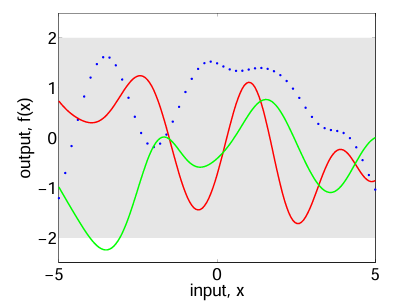
\includegraphics[width=1\linewidth]{figures/prior.png}
        \caption{prior}
        \label{fig:prior}
    \end{subfigure}
    \hfill
    \begin{subfigure}[b]{0.5\textwidth}
        \centering
        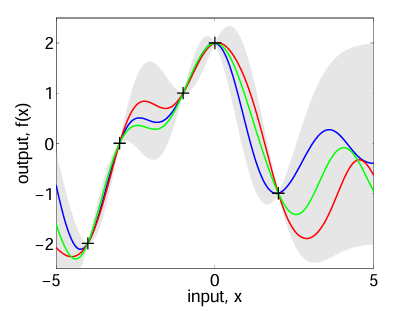
\includegraphics[width=1\linewidth]{posterior.png}
        \caption{posterior}
        \label{fig:posterior}
    \end{subfigure}
    \caption{Panel (a) displays three functions drawn at random from a GP prior. The dots represent values of \(y\) actually generated, while the other functions have been drawn as lines by connecting a large number of evaluated points.Panel (b) illustrates three random functions drawn from the posterior, i.e., the prior conditioned on the five noise-free observations indicated. In both plots, the shaded area represents the pointwise mean plus and minus two times the standard deviation for each input value (corresponding to the 95\% confidence region), for the prior and posterior, respectively \cite{williams2006gaussian}.}
    \label{fig:prior_posterior}
\end{figure}

\subsubsection{Posterior Distribution}
To predict function values for all inputs considering observations, the equation 
\begin{equation}
    f(X^*) = X^T_*\mathbf{w}
\end{equation} 
is used, where \( X^* \) denotes a matrix consisting of test points \( \mathbf{x^*} \) such that \( X^* \in \mathbb{R}^{D} \), \( X^* = [\mathbf{x^*_1, \ldots, x^*_s}] \). The posterior distribution of weights, denoted as $w$, is used to predict function values for all inputs considering observations. This distribution is obtained through Bayes' rule, where the posterior ($p(a|b)$) is proportional to the likelihood ($p(b|a)$) multiplied by the prior ($p(a)$) and normalized by the marginal likelihood ($p(b)$). In the context of the posterior distribution of weights, Bayes' rule can be rewritten as:
\begin{equation}\label{eq:bayes_rule}
    p(\mathbf{w}|\mathbf{y},X) = \frac{p(\mathbf{y}|X,\mathbf{w}) \cdot p(\mathbf{w})}{p(\mathbf{y}|X)}
\end{equation}

\begin{figure}
    \centering
    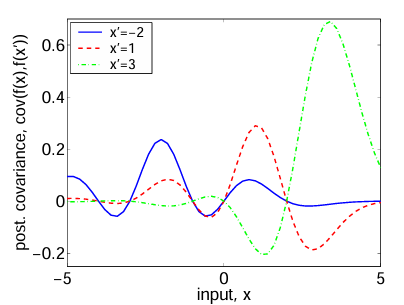
\includegraphics[width=0.6\linewidth]{figures/posterior_cov.png}
    \caption{The posterior covariance illustrates the covariance between \( f(x) \) and \( f(x') \) for the same data, with three different values of \( x' \). Notably, the covariance is high at points close to each other, diminishes to zero at the training points (where variance is absent due to the noise-free process), and subsequently becomes negative. This variation occurs because if the smooth function happens to be below the mean on one side of a data point, it is inclined to surpass the mean on the opposite side, resulting in a change in the sign of the covariance at the data points. In contrast, the prior covariance exhibits a Gaussian shape and remains non-negative. \cite{williams2006gaussian}.}
    \label{fig:Post_cov}
\end{figure}

The prior represents the model weights' beliefs without observations, often assumed as a Gaussian distribution with zero mean and covariance matrix as shown in Equation ( \ref{eq:prior_function}). The likelihood \( p(y | X, w) \) is the probability density function of the observations given the inputs and model weights, which can be determined using Equation (\ref{eq:latent_function}). 

\begin{equation}\label{eq:likelihood}
     p(\mathbf{y} | X, \mathbf{w}) = \mathcal{N}(X^T\mathbf{w}, \sigma^2_n I)
\end{equation}

By combining the prior Equation (\ref{eq:prior_function}) and likelihood Equation (\ref{eq:likelihood}), the posterior distribution of weights given observations  can be determined by their multiplication as shown in Equation \ref{eq:posterior}

\begin{equation}\label{eq:posterior}
    p(\mathbf{w} | \mathbf{y}, X) \propto p(\mathbf{y} | X, \mathbf{w}) \cdot p(\mathbf{w})
\end{equation}

The marginal likelihood is independent of \( w \) and just a normalization constant which does not influence the shape of the distribution. By substituting $A = \sigma^{-2}_n XX^T + \Sigma^{-1}_p$ and adding the terms $\pm \sigma^{-2}_n y^TX^TA^{-1}A^{-1}Xy \sigma^{-2}$ to the exponent, the equation can be rewritten as:
\begin{equation}
    p(\mathbf{w|y},X) \propto \exp\left(-\frac{1}{2} \mathbf{w}^T \left(\sigma^{-2}_n A^{-1}X\mathbf{y}\right) - \frac{1}{2} \sigma^{-2}_n y^TX^TA^{-1}A^{-1}X\mathbf{y}\right),
\end{equation}

where \( \alpha = \sigma^{-2}_n (A^{-1} y^T y - y^T X A^{-1}A^{-1} X^T y) \) is independent of \( w \) and hence also a scaling factor. Finally, the posterior is distributed according to:
\begin{equation}\label{eq:posterior_distrubtion}
     p(\mathbf{w | y}, X) = \mathcal{N}\left(\frac{1}{\sigma^2_n} A^{-1} X\mathbf{y}, A^{-1}\right)
\end{equation}



\subsubsection{Prediction}
When making predictions using Gaussian processes (GPs), incorporating observed data is crucial. For noise-free observations $\{(\mathbf{x_i}, f_i) | i = 1,...,n\}$, the joint distribution of training outputs $f$ and test outputs $f^*$ under the prior is given by:
\begin{equation}\label{eq:noisefree_joint_distrubtion}
    \begin{bmatrix}f, f^*\end{bmatrix} \sim \mathcal{N} \left(0, \begin{bmatrix} K(X,X) & K(X,X^*) \\ K(X^*,X) & K(X^*,X^*) \end{bmatrix} \right)
\end{equation}

To obtain the posterior distribution over functions, we condition this joint prior distribution on the observed data points. The resulting posterior distribution is expressed as:
\begin{equation}\label{noisefree_predictive_distrbution}
    f^* | X^*, X, f \sim \mathcal{N} \left( K(X^*,X)K(X,X)^{-1}f, K(X^*,X^*) - K(X^*,X)K(X,X)^{-1}K(X,X^*) \right)
\end{equation}

This enables sampling function values $f^*$ from the joint posterior distribution by evaluating the mean and covariance matrix.

Prediction with noisy observations incorporates additive independent identically distributed Gaussian noise. The joint distribution of observed target values and function values at test locations under the prior is given by:

\begin{equation}\label{eq:noisy_joint_distrubtion}
     \begin{bmatrix}\mathbf{y}, f^* \end{bmatrix} \sim \mathcal{N} \left(0, \begin{bmatrix} K(X,X) + \sigma^2_n I & K(X,X^*) \\ K(X^*,X) & K(X^*,X^*) \end{bmatrix} \right)
\end{equation}

The predictive equations for GP regression are:
\begin{align}\label{noisy_predictive_distrbution}
\bar{f}^* &= K(X^*,X)[K(X,X) + \sigma^2_n I]^{-1}y \\
\text{cov}(f^*) &= K(X^*,X^*) - K(X^*,X)[K(X,X) + \sigma^2_n I]^{-1}K(X,X^*)
\end{align}

These equations provide mean predictions and uncertainties for test targets.

\subsection{Extension to Non-Linear Functions}\label{sec:section2.2}
Gaussian processes can be used for both linear regression,  restricting them to linear regression means that it won't capture nonlinear relationships between variables effectively. If the relationship between the input and output variables is nonlinear, using a linear model might result in poor predictions and biased estimates. Since the order of the target function is generally unknown, direct application of raw inputs is not effective.  To overcome this problem, the idea is to transform the inputs into a higher dimensional space via basis functions $\psi(x)$, $\psi : \mathbb{R}^D \rightarrow \mathbb{R}^N$, where $N \gg D$, and then apply the linear regression model. Thus the linear regression model Equation \ref{eq:latent_function} is reformulated such that 
\begin{equation}\label{eq:non_linear_regression_model}
f(x) = \psi(x)w, \quad 
\end{equation}

Accordingly, the predictive distribution is given by:

\begin{equation}\label{eq:Nl_pd}
p(f^*|X^*,X,\mathbf{y}) = \mathcal{N} \left( \frac{1}{\sigma_n^2} \Psi(X^*)^T A^{-1} \Psi(X) \mathbf{y}, \frac{1}{\sigma_n^2} \Psi(X^*)^T A^{-1} \Psi(X^*) \right)
\end{equation}
With $A = \sigma^{-2} n \Psi(X)\Psi(X)^T + \Sigma_p$, can be rearranged as shown in \cite{williams2006gaussian}, such that

\begin{equation}\label{eq:NL_pd_arranged}
p(f^*|X^*, X, y) = \mathcal{N}(\Psi_*^T \Sigma_p \Psi_K + \sigma^2_n I)^{-1} y, \Psi_*^T \Sigma_p \Psi_* - \Psi_*^T \Sigma_p \Psi_K + \sigma^2_n I)^{-1} \Psi_*^T \Sigma_p \Psi_*,
\end{equation}

where $K = \Psi_*^T \Sigma_p \Psi$. The Equation \ref{eq:NL_pd_arranged} explicitly depends on basics functions $\psi$ i.e the feature space appears only in the form of $\Psi^*\Sigma_p\Psi^*$, $\Psi^*\Sigma_p\Psi$, and $\Psi\Sigma_p\Psi$. the basis functions $\psi$ explicitly is not feasible. Thus, defining $\varphi(x) = \Sigma_{1/2}^p \psi(x)$ (notice that $\Sigma_p$ is positive definite), the expressions can be substituted by $\varphi(x) \varphi(x)^T$. So $\langle \varphi(x), \varphi(x)^T \rangle$ can be replaced by kernel function $k(x,x^T)$ using Mercer’s theorem \cite{kanagawa2018}. The kernel matrices $K(\cdot,\cdot)$ which are given by:

\begin{equation}\label{eq:kernal_f}
    K(X,Y) =
\begin{pmatrix}
k(X_1,Y_1) & \cdots & k(X_1,Y_M) \\
\vdots & \ddots & \vdots \\
k(X_N,Y_1) & \cdots & k(X_N,Y_M)
\end{pmatrix}
\end{equation}

Substituting kernal function (\ref{eq:kernal_f}) into (\ref{eq:NL_pd_arranged})

% \begin{equation}\label{eq: NL_pd_implicit}
% \begin{aligned}
% p(f^*|X^*,X,y) & = \mathcal{N}\left(K(X^*,X) [K(X,X) + \sigma^2_n I]^{-1} y, \right. \nonumber \\
% & \qquad \left. K(X^*,X^*) - K(X^*,X)[K(X,X) + \sigma^2_n I]^{-1} K(X,X^*)\right).
% \end{aligned}
% \end{equation}

\begin{equation}\label{eq: NL_pd_implicit}
\begin{aligned}
p(f^*|X^*,X,\mathbf{y}) & = \mathcal{N} (K(X^*,X) [K(X,X) + \sigma^2_n I]^{-1} y,  \nonumber \\
& \qquad  K(X^*,X^*) - K(X^*,X)[K(X,X) + \sigma^2_n I]^{-1} K(X,X^*)).
\end{aligned}
\end{equation}

This new formalism depends only implicitly on the basis functions via the kernel matrices and is preferred because determining the basis functions explicitly is quite hard Equation \ref{eq: NL_pd_implicit}


\textbf{Assumption 2.1:}\label{as:assumption2.1} The objective function $f$ is a member of a reproducing kernel Hilbert space (RKHS), with known kernel function $k(\cdot,\cdot) : X \times X \rightarrow \mathbb{R}$ and bounded norm $\|f\|_H^2 \leq B$. 


Assumption 2.1 is necessary to ensure the applicability of Gaussian processes \cite{williams2006gaussian}, which can be seen in the modified problem description (\ref{eq:non_linear_regression_model}) where $f(x)$ is defined as the linear combination of the basis functions $\psi(x)$. The bound on $\|f\|_H$ imposes a complexity and magnitude condition on the RKHS; if $\|f\|_H$ gets smaller, $f$ gets smoother (less complex) \cite{kanagawa2018}. One might imagine that a function assumed to have infinite complexity would not be feasible because the uncertainty for the predictive distribution would be infinite for all $X \setminus O$.


\subsection{Long-term Prediction}\label{sec:section2.3}
When the input \( X^* \) (we employ lower-case \( x^* \) for a single test input and upper-case \( X* \) for several test inputs) is a deterministic input, the mean and covariance of the prediction are calculated according to Equation (\ref{eq:noisefree_joint_distrubtion}). However, if the input itself is Gaussian, \( X \sim \mathcal{N}( \bar{x^*}, \Sigma_x^* ) \), the predictive distribution becomes:

\begin{equation}\label{eq:single_prediciton}
p(f^*|\mu_x^*, \Sigma_x^* , \mathbf{D}) = \int p(f^*|X^*, \mathbf{D}) \cdot p(X^*|\Sigma_x^* , \mathbf{D}) \, dx^* \quad
\end{equation}

The integral in Equation (\ref{eq:single_prediciton}) is analytically intractable \cite{hewing2017cautious}. To address this, various methods have been developed to approximate the posterior distribution \cite{girard2003gaussian}. One approach is to approximate the integral numerically using Monte-Carlo methods \cite{girard2002gaussian}. Alternatively, the posterior distribution \( p(f|x, \mathbf{X}, \mathbf{D}) \) can be approximated as a Gaussian by calculating its mean and variance. Several methods exist for this Gaussian approximation, such as Moment Matching and linearization of the posterior GP mean function\cite{marc2015robotics}. Moment Matching computes the first two moments of the predictive distribution exactly, whereas linearization provides a computationally efficient approximation by explicitly linearizing the posterior GP. In this thesis, we will focus on the Moment Matching Gaussian approximation.


% The integral in Equation(\ref{eq:single_prediciton}) is analytically intractable \cite{hewing2017cautious}. Several methods exist for approximating the posterior distribution \cite{girard2003gaussian}. One possible solution is to approximate the integral numerically by a Monte-Carlo approximation \cite{girard2002gaussian}. Another solution is to approximate the posterior distribution \( p(f|x, \mathbf{X}, \mathbf{D}) \) as a Gaussian by calculating its mean and variance. There are several Gaussian mean, and variance approximation methods such as Moment Matching, and linearization of the posterior GP mean function. While moment matching computes the first two moments of the predictive distribution exactly, their approximation by explicit linearization of the posterior GP is computationally advantageous. We will focus on the Moment Matching Gaussian approximation in this thesis. 

As shown in \cite{quignonero2003propagation}, it is possible to compute the mean and variance analytically in the case of a Gaussian kernel function. The main results are presented here. Following the law of iterated expectations, for target dimensions \( a = 1,..., D \) we obtain the predictive mean:

\begin{equation}\label{eq:mu}
\begin{aligned}
\mu_t^a & =\mathbb{E}_{\tilde{\boldsymbol{x}}_{t-1}}\left[\mathbb{E}_{f_a}\left[f_a\left(\tilde{\boldsymbol{x}}_{t-1}\right) \mid \tilde{\boldsymbol{x}}_{t-1}\right]\right]=\mathbb{E}_{\tilde{\boldsymbol{x}}_{t-1}}\left[m_{f_a}\left(\tilde{\boldsymbol{x}}_{t-1}\right)\right] \\
& =\int m_{f_a}\left(\tilde{\boldsymbol{x}}_{t-1}\right) \mathcal{N}\left(\tilde{\boldsymbol{x}}_{t-1} \mid \tilde{\boldsymbol{\mu}}_{t-1}, \tilde{\boldsymbol{\Sigma}}_{t-1}\right) d \tilde{\boldsymbol{x}}_{t-1} \\
& =\boldsymbol{\beta}_a^T \boldsymbol{q}_a 
% \boldsymbol{\beta}_a & =\left(\boldsymbol{K}_a+\sigma_{w_a}^2\right)^{-1} \boldsymbol{y}_a
\end{aligned}
\end{equation}
where,
\begin{equation}\label{eq:beta}
    \boldsymbol{\beta}_a =\left(\boldsymbol{K}_a+\sigma_{w_a}^2\right)^{-1} \boldsymbol{y}_a
\end{equation}

with $\boldsymbol{q}_a=\left[q_{a_1}, \ldots, q_{a_n}\right]^T$. The entries of $\boldsymbol{q}_a \in \mathbb{R}^n$ are computed using standard results from multiplying and integrating over Gaussians and are given by

\begin{equation}\label{eq:mu_qa}
\begin{aligned}
q_{a_i} & =\int k_a\left(\tilde{\boldsymbol{x}}_i, \tilde{\boldsymbol{x}}_{t-1}\right) \mathcal{N}\left(\tilde{\boldsymbol{x}}_{t-1} \mid \tilde{\boldsymbol{\mu}}_{t-1}, \tilde{\boldsymbol{\Sigma}}_{t-1}\right) d \tilde{\boldsymbol{x}}_{t-1} \\
& =\sigma_{f_a}^2\left|\tilde{\boldsymbol{\Sigma}}_{t-1} \boldsymbol{\Lambda}_a^{-1}+\boldsymbol{I}\right|^{-\frac{1}{2}} \exp \left(-\frac{1}{2} \boldsymbol{\nu}_i^T\left(\tilde{\boldsymbol{\Sigma}}_{t-1}+\boldsymbol{\Lambda}_a\right)^{-1} \boldsymbol{\nu}_i\right),
\end{aligned}
\end{equation}

where we define
\begin{equation}\label{eq:difference_vi}
    \nu_i:=\left(\tilde{\boldsymbol{x}}_i-\tilde{\boldsymbol{\mu}}_{t-1}\right)
\end{equation}
is the difference between the training input $\tilde{\boldsymbol{x}}_i$ and the mean of the test input distribution $p\left(\boldsymbol{x}_{t-1}, \boldsymbol{u}_{t-1}\right)$.

Computing the predictive covariance matrix $\mathbf{\Sigma}_{\Delta} \in \mathbb{R}^{D \times D}$ requires us to distinguish between diagonal elements $\sigma_{a a}^2$ and off-diagonal elements $\sigma_{a b}^2, a \neq b$ : Using the law of total (co-)variance, we obtain for target dimensions $a, b=$ $1, \ldots, D$
\begin{equation}\label{eq:sigma_aa}
\sigma_{a a}^2  =\mathbb{E}_{\overline{\boldsymbol{x}}_t}\left[\operatorname{var}_f\left[\Delta_a \mid \tilde{\boldsymbol{x}}_t\right]\right]+\mathbb{E}_{f, \overline{\boldsymbol{x}}_t}\left[\Delta_a^2\right]-\left(\boldsymbol{\mu}_{\Delta}^a\right)^2,
\end{equation}
\begin{equation}\label{eq:sigma_ab}
    \sigma_{a b}^2 =\mathbb{E}_{f, \overline{\boldsymbol{x}}_t}\left[\Delta_a \Delta_b\right]-\boldsymbol{\mu}_{\Delta}^a \boldsymbol{\mu}_{\Delta}^b, \quad a \neq b,
\end{equation}

respectively, where $\mu_{\Delta}^a$ is known from (\ref{eq:mu}). The off-diagonal terms $\sigma_{a b}^2$ do not contain the additional term $\mathbb{E}_{\overline{\boldsymbol{x}}_t}\left[\operatorname{cov}_f\left[\Delta_a, \Delta_b \mid \tilde{\boldsymbol{x}}_t\right]\right]$ because of the conditional independence assumption of the GP models: Different target dimensions do not covary for given $\tilde{\boldsymbol{x}}_t$.

We start the computation of the covariance matrix with the terms that are common to both the diagonal and the off-diagonal entries: With $p\left(\tilde{\boldsymbol{x}}_t\right)=\mathcal{N}\left(\tilde{\boldsymbol{x}}_t \mid \tilde{\boldsymbol{\mu}}_t, \tilde{\boldsymbol{\Sigma}}_t\right)$ and the law of iterated expectations, we obtain
\begin{equation}\label{eq:Eab}
\begin{aligned}
\mathbb{E}_{f, \overline{\boldsymbol{x}}_t}\left[\Delta_a \Delta_b\right] & =\mathbb{E}_{\overline{\boldsymbol{x}}_t}\left[\mathbb{E}_f\left[\Delta_a \mid \tilde{\boldsymbol{x}}_t\right] \mathbb{E}_f\left[\Delta_b \mid \tilde{\boldsymbol{x}}_t\right]\right] \\
& \stackrel{(6)}{=} \int m_f^a\left(\tilde{\boldsymbol{x}}_t\right) m_f^b\left(\tilde{\boldsymbol{x}}_t\right) p\left(\tilde{\boldsymbol{x}}_t\right) \mathrm{d} \tilde{\boldsymbol{x}}_t
\end{aligned}
\end{equation}

because of the conditional independence of $\Delta_a$ and $\Delta_b$ given $\tilde{\boldsymbol{x}}_t$. Using the definition of the GP mean function, we obtain

\begin{equation}\label{eq:Eab_beta}
    \mathbb{E}_{f, \overline{\boldsymbol{x}}_t}\left[\Delta_a \Delta_b\right]=\boldsymbol{\beta}_a^{\top} \boldsymbol{Q} \boldsymbol{\beta}_b,
\end{equation}
\begin{equation}\label{eq:Q_integral}
    \boldsymbol{Q}:=\int k_a\left(\tilde{\boldsymbol{x}}_t, \tilde{\boldsymbol{X}}\right)^{\top} k_b\left(\tilde{\boldsymbol{x}}_t, \tilde{\boldsymbol{X}}\right) p\left(\tilde{\boldsymbol{x}}_t\right) \mathrm{d} \tilde{\boldsymbol{x}}_t .
\end{equation}

Using standard results from Gaussian multiplications and integration, we obtain the entries $Q_{i j}$ of $Q \in \mathbb{R}^{n \times n}$
\begin{equation}\label{eq:Qij}
    Q_{i j}=|\boldsymbol{R}|^{-\frac{1}{2}} k_a\left(\tilde{\boldsymbol{x}}_i, \tilde{\boldsymbol{\mu}}_t\right) k_b\left(\tilde{\boldsymbol{x}}_j, \tilde{\boldsymbol{\mu}}_t\right) \exp \left(\frac{1}{2} \boldsymbol{z}_{i j}^{\top} \boldsymbol{T}^{-1} \boldsymbol{z}_{i j}\right)
\end{equation}

where we define
$\qquad \boldsymbol{R}  :=\tilde{\boldsymbol{\Sigma}}_t\left(\boldsymbol{\Lambda}_a^{-1}+\boldsymbol{\Lambda}_b^{-1}\right)+\boldsymbol{I}, \qquad \boldsymbol{T}:=\boldsymbol{\Lambda}_a^{-1}+\boldsymbol{\Lambda}_b^{-1}+\tilde{\boldsymbol{\Sigma}}_t^{-1}, \\ \boldsymbol{z}_{i j} :=\boldsymbol{\Lambda}_a^{-1} \boldsymbol{\nu}_i+\boldsymbol{\Lambda}_b^{-1} \boldsymbol{\nu}_j,$


with $\nu_i$ defined in (\ref{eq:difference_vi}). Hence, the off-diagonal entries of $\Sigma_{\Delta}$ are fully determined by (\ref{eq:mu})-(\ref{eq:difference_vi}), (\ref{eq:sigma_ab}), and (\ref{eq:Eab_beta})-(\ref{eq:Qij}).

From (\ref{eq:sigma_aa}), we see that the diagonal entries contain the additional term
\begin{equation}\label{eq:E_xa}
    \mathbf{E}_{\overline{\boldsymbol{x}}_t}\left[\operatorname{var}_f\left[\Delta_a \mid \tilde{\boldsymbol{x}}_t\right]\right]=\sigma_{f_a}^2-\operatorname{tr}\left(\left(\boldsymbol{K}_a+\sigma_{w_a}^2 \boldsymbol{I}\right)^{-1} \boldsymbol{Q}\right)+\sigma_{w_a}^2
\end{equation}

with $Q$ given in (\ref{eq:Qij}) and $\sigma_{w_a}^2$ being the system noise variance of the $a$ th target dimension. This term is the expected variance of the function, under the distribution $p\left(\tilde{\boldsymbol{x}}_t\right)$.

The final covariance matrix is given by 
\begin{equation}
    \sum (:) = 	\begin{bmatrix}
                        \sigma_{a a}^2 & \sigma_{a b}^2 &......\\
                        \sigma_{a b}^2 & \sigma_{b b}^2 &......\\
                        .&.& ......\\
                        .&.& ......\\
                        \end{bmatrix}_{DxD}
\end{equation}


\subsection{Optimization of the Hyperparameters}\label{sec:optimize_hy}

To ensure accurate predictions, selecting appropriate hyperparameters is crucial. However, in the case of a black-box system, precise information about these hyperparameters is often unavailable, necessitating the use of computationally efficient methods for optimization. In \cite{williams2006gaussian}, two such methods are introduced: maximizing the marginal likelihood (Bayesian model selection) and cross-validation. Hyperparameters are typically determined using available training data \( \mathcal{D} \), rather than relying solely on prior knowledge or physical insight, which can be challenging. Given a prior probabilistic belief of the hyperparameters' distribution \( p(\theta) \) (often assumed to be uniform), the goal is to infer the hyperparameters' posterior distribution \( p(\theta|W,z) \) using Bayes' theorem:


\begin{figure}
    \centering
    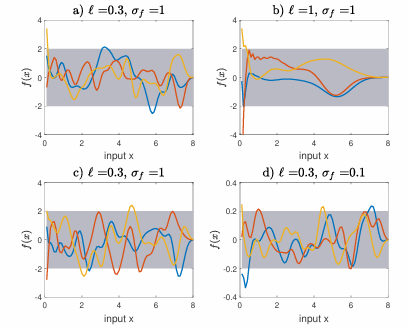
\includegraphics[width=0.65\linewidth]{figures/opt_hyp_prior.png}
    \caption{Three samples are drawn from the prior with different sets of hyperparameters. Figures (a) and (b) demonstrate the impact of changing the lengthscale, while Figures (c) and (d) illustrate the effect of varying the signal standard deviation \( f \). The uncertainty is depicted by the 95\% confidence interval, shaded in gray \cite{rezvani2019gaussian}. }
    \label{fig:opt_hyp_prior}
\end{figure}






\begin{equation}\label{eq: marginal_likelihood}
\begin{aligned}
p(w|y,X,\theta) &= \frac{p(y|X,w,\theta) \cdot p(w|\theta)}{p(y|X,\theta)}, \\
p(y|X,\theta) &= \int p(y|X,w,\theta) \cdot p(w|\theta) \, dw.
\end{aligned}
\end{equation}




The optimal solution would be a predictive distribution without dependency on the hyperparameters. By marginalization of \( \theta \), a hyperparameter-independent formalism can be obtained:

\begin{equation}\label{eq: predictive_distribution}
p(f^*|y,X,X^*) = \int p(f^*|y,\theta,X,X^*) \cdot p(y|\theta,X,X^*) \cdot p(\theta|X,X^*) \, d\theta.
\end{equation}

Unfortunately, this integral is not analytically tractable, as \( p(f^*|y,\theta,X,X^*) \) and \qquad a \( p(y|\theta,X,X^*) \) have non-trivial dependencies on \( \theta \). Several methods exist to estimate the integral, such as Hamiltonian Monte Carlo (HMC), Bayesian Monte Carlo (BMC), and Sequential Monte Carlo (SMC).

An alternative approach to approximate \eqref{eq: predictive_distribution} is by maximizing the second-level marginal likelihood (ML-II) given by \eqref{eq: marginal_likelihood}. As shown in previous work, finding the hyperparameters \( \theta_{\text{max}} \) that maximize \( p(y|X,\theta) \) leads to:

\[
p(f^*|y,X,X^*) \approx p(f^*|\theta_{\text{max}},y,X,X^*).
\]


\begin{figure}
    \centering
    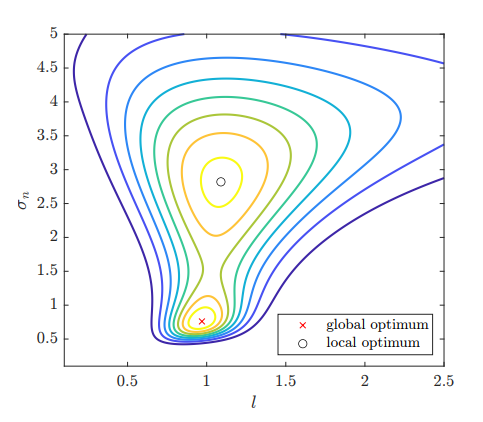
\includegraphics[width=0.75\linewidth]{figures/Contour_hyp.png}
    \caption{Contour of the marginal likelihood depending on the length scale \( l \) and noise \( \sigma_n \) \cite{Lubsen2022}.}
    \label{fig:opt_hyp_post}
\end{figure}

This method offers the advantage of analytically tractable integration. Gradient-based algorithms are typically used for maximization due to the computational efficiency of determining the partial derivatives of the likelihood with respect to \( \theta \). However, the non-convex nature of the marginal likelihood surface can lead to overfitting or underfitting. Additionally, gradient-based optimization is highly sensitive to initial values.

The contour of the marginal likelihood as a function of the length scale and noise is illustrated in Figure \ref{fig:opt_hyp_post}, showing both local and global minima. Global optimization using the hyperparameters at the global optimum results in preferable predictions compared to local minima, where observations may be misinterpreted as noise.

Reasonable hyperparameter selection is crucial, and alternative methods such as global optimizers like Dividing Rectangles (DIRECT) can be utilized to mitigate sensitivity to initial values. If the noise level is known, fixing the respective hyperparameter during optimization can prevent misinterpretation of observations.



% \begin{equation}
%     p(\theta|W,z) = \frac{p(z|W,\theta) p(\theta)}{p(z|W)}
% \end{equation}

% Here, \( p(z|W,\theta) \) is the likelihood and \( p(z|W) \) is the marginal likelihood (or evidence). However, in most cases, these integrals are intractable and numerical approximations are necessary. One approach is to maximize the likelihood \( p(z|W,\theta) \)[\cite{roberts2013gaussian}], which is effective when the likelihood is highly peaked, as is often the case with a large training dataset. A common method is to compute a point estimate of the most likely hyperparameters by maximizing the log likelihood:
% \begin{equation}
%     \log(p(z|W,\theta)) = -\frac{1}{2}z^T K^{-1} z - \frac{1}{2} \log(\text{det}(K)) - \frac{n}{2} \log(2\pi)
% \end{equation}

% with respect to \( \theta \) (see, e.g., [\cite{kocijan2016modelling}]).

% In the context of Gaussian processes (GPs), the term "learning" is used ambiguously, referring both to the inference step from prior to posterior and the optimization of hyperparameters. However, both steps are essential. GPs can be distinguished based on whether learning is performed offline or online during operation. This can involve offline inference and hyperparameter optimization [\cite{ostafew2014learning,likar2007predictive,kocijan2003predictive}], online inference and hyperparameter optimization [\cite{ortmann2017gaussian,murraysmith2003adaptive,klenske2016gaussian}], or a hybrid approach that combines offline hyperparameter optimization with online inference updates based on newly available training data [\cite{hewing2017cautious,ostafew2016learning,ostafew2014learning}]. This work considers the latter case.


% In hierarchical Bayesian models, the lowest level comprises the model parameters \( w \), given the hyperparameters \( \theta \) as introduced in Section 2.3, which define the distribution of parameters at the first level. Starting from the bottom level, the posterior over parameters is defined in (2.5) and can be expressed as
% \[
% p(w|y,X,\theta) = \frac{p(y|X,w,\theta) \cdot p(w|\theta)}{p(y|X,\theta)}
% \]
% by conditioning with \( \theta \). The denominator represents the marginal likelihood and is independent of the parameters, determined by integrating the product of the likelihood and the prior over model parameters as shown in (2.33). Ideally, the predictive distribution would be independent of the hyperparameters. However, marginalizing \( \theta \) to obtain a hyperparameter-independent formulation leads to an analytically intractable integral as shown in (2.34). Various methods, such as Hamiltonian Monte Carlo (HMC), Bayesian Monte Carlo (BMC), and Sequential Monte Carlo (SMC), can be employed to estimate this integral.

% Alternatively, approximating (2.34) can be achieved by maximizing the second-level marginal likelihood (ML-II, (2.33)). This involves finding \( \theta_{\text{max}} = \text{argmax























% The following hints are taken from the Writing-Coach, developed at the Essen University, \cite{BuBiPo00}. On that German homepage
% \begin{center}
% \href{http://www.uni-essen.de/schreibwerkstatt/trainer}
% {http://www.uni-essen.de/schreibwerkstatt/trainer}.
% \end{center} 
% much more can be found about scientific writing in German. Nevertheless lots of help in English can be found on the Internet.
% Also check out \cite{Fe13}.


% \subsection{Correctness}

% Your writing should be as accurate as possible. Do not use colloquial language, neither filler or vogue words.
% As such, technical/scientific writing style serves a purpose: to transport information as efficiently as possible.

% Respect the rules of grammar, spelling and punctuation. Text, sentences or words used in the wrong context, can 
% lead to misunderstandings or may be hard to understand. The sentences in text documents need to be complete.

% It is clear that the results of your work, e.g., experiments, are documented correctly, even though they might have had unexpected outcomes.
% Otherwise you do not only cause harm to you but any further research. 


% \subsection{Comprehensibility}

% Correctness does not imply comprehensibility. Look at your text from the readers point of view: Consider his or her position, previous knowledge
% and attitude. Formulate as precisely as possible but not more than necessary. Therefore, 
% \begin{itemize}
%     \item choose words, that are known;
%     \item use words that are probably unknown, such that their meaning can be deduced from the context, or explain or define them;
%     \item do not construct deeply nested sentences.
% \end{itemize}


% \subsection{Line of Reasoning}

% The line of reasoning depends on your topic and the type of text. To get a general structure, address the following six questions:

% \begin{enumerate}
%     \item What is the purpose of the text?
%     \item What is the content? What is to be included and why?
%     \item What is not (anymore) part of the content? What is to be excluded?
%     \item Which parts of the contents belong together? What is the structure of the topic?
%     \item What part of the contents is suited to conclude with?
%     \item What part of the contents is suited to start with?
% \end{enumerate}

% These questions show the possibilities for a line of reasoning. They show that---even for one type of text with one purpose---different lines of reasoning are possible. 
% To choose one, it is important to analyze the topic and the content.


% \subsection{References}

% One of the most important differences between scientific writing and writing other texts is citing the references used for your work. 
% Before starting to write your scientific text, you have probably been reading (or you still are) a lot of books, articles, conference proceedings, 
% manuals, etc. Some may turn out to be of no interest, but some may give you the fundamental ideas. 

% In any case, you have to cite those references you made use of and point out all parts of your work that are based on results of others 
% (those could even be your own results, if you have already published some work).

% The citation normally follows a sentence, separated by a comma. In general you don't use direct quotes in engineering sciences, but repeat the contents in your own words for better understandability
% and make clear from the proper positioning of the citation---and if necessary an additional clarifying sentence---that you are referring to other work.

% The bibliography follows at the end of your work, prior to the appendix. All your cited references are listed here. \LaTeX\ offers many ways to generate
% such a listing automatically, which will be explained in the next chapter.

% \subsection{Structure}

% Start your scientific text with an introduction, that
% \begin{itemize}
%     \item introduces the subject,
%     \item specifies the topic,
%     \item reflects on the problem that you are going to consider,
%     \item defines the purpose of the work,
%     \item explains the line of reasoning
%     \item sketches the structure of the work.
% \end{itemize}

% Keep in mind that there are some readers that only read the introduction and conclusion of your work
% and base their decision on whether the work bears any interest for them only on these parts. To make that decision,
% they need to get all relevant information from those two chapters. Hint: Look at other work with a focus on that question.

% The main part of your work should be structured as well, however here there are no general rules. The order of your
% chapters depends, if your focus was either on theoretic, methodical or experimental work. Think about a weighting for each
% chapter. What is reflected in volume and does not necessarily need to be proportional to the amount of time, you have 
% spent to solve the respective problems. Sometimes it takes one week to debug a piece of code, which nevertheless should not be explained excessively.

% Your work concludes with a summary of your results. Therefore have a look at your introduction: how you have specified the problem there and does it
% match with your results. Do not present any further results here that have been not presented in the main part. As such, always clearly
% separate the presentation and the discussion of results.

% Finally, you end with an outlook that points out open questions. What should be further analyzed and what are possible followup projects?
% Do not be afraid to point out questions that came to your mind during your research, but you did not have time to properly answer. 
% A good thesis may raise more questions than it clarifies.}		%
	{\section {Der wissenschaftliche Schreibstil}
\label{a:stil}

Die nachfolgenden Unterpunkte sind dem an der Universität Essen
entwickelten Schreibtrainer entnommen, \cite{BuBiPo00}. Dort kann
ein Vielfaches an Informationen mehr rund um das Schreiben
nachgeschlagen werden, was bitte als Ermunterung verstanden werden
soll! Im Internet findet man den Schreibtrainer unter der
Web-Adresse

\begin{center}
\href{http://www.uni-essen.de/schreibwerkstatt/trainer}
{http://www.uni-essen.de/schreibwerkstatt/trainer}.
\end{center}


\subsection{Korrektheit}

Der sprachliche Ausdruck sollte so treffend wie möglich sein. Die
Wörter dürfen weder umgangssprachlich noch Modewörter oder
Füllwörter sein, hier können Wörterbücher eine Hilfe sein.

Die Regeln der Grammatik, der Rechtschreibung und der
Zeichensetzung sind zu beachten. Texte, Sätze oder Wörter, die
sprachlich falsch sind, können für den Leser missverständlich oder
ärgerlich sein. Die Sätze in Schrifttexten müssen vollständig
sein.

Dass die eigentlichen Ergebnisse (z.B.\ Experimente) auch korrekt
wiedergegeben werden müssen (auch wenn es nicht so schön aussieht,
wie eigentlich erwartet), ist selbstverständlich. Wer hier nicht
wahrhaftig ist, schadet nicht nur sich selbst, sondern in gewisser
Weise der ganzen Weiterentwicklung.


\subsection{Verständlichkeit}

Nicht alles, was richtig ist, ist auch  verständlich. Die
Verständlichkeit eines Textes muss aus der Perspektive des Lesers
beurteilt werden: Seine Position, sein Vorwissen, sein
Aufnahmevermögen sind zu bedenken. Formulierungen sollten so genau
wie möglich, aber nicht genauer als nötig sein. Entsprechend sind
\begin{itemize}
    \item solche Wörter zu wählen, die bekannt sind;
    \item vermutlich unbekannte, klärungsbedürftige Wörter so einzubinden,
        dass ihre Bedeutung sich aus dem Zusammenhang erschließt,
        sie zu definieren oder zu erklären;
    \item Sätze weder nebeneinander zu stellen noch zu verschachtelt zu bauen und
    \item abhängig von der Textsorte und der Länge des Textes Textkommentare einzufügen.
\end{itemize}


\subsection{Argumentationweise}

Der Gang einer Argumentation ist immer vom Thema und von der
Textsorte abhängig. Um zunächst einen groben Textverlauf
festzulegen, sollte man die folgenden sechs Fragen klären:

\begin{enumerate}
    \item Was ist das Textziel?
    \item Was ist der Textinhalt? Was wird warum eingegrenzt?
    \item Was gehört nicht (mehr) zum Textinhalt, was wird ausgegrenzt?
    \item Welche Teile des Textinhaltes gehören wie zusammen, wie ist die
        Struktur des Themas?
    \item Welcher Teil des Textinhalts ist ein geeigneter Zielpunkt?
    \item Welcher Teil des Textinhalts ist ein geeigneter
        Anfangspunkt?
\end{enumerate}

Die sechs Fragen skizzieren die Möglichkeiten, die für eine
Argumentation bestehen, sie legen den roten Faden fest. Sie zeigen
deutlich, dass - selbst bei übereinstimmender Textsorte und
übereinstimmendem Textziel - viele unterschiedliche Texte
(Textverläufe) zu einem Thema denkbar sind. Um sich bewusst für
einen Verlauf entscheiden zu können, ist es wichtig, das Thema und
damit auch den Textinhalt genau zu analysieren.


\subsection{Quellenangaben}


Mit der wichtigste Unterschied zwischen wissenschaftlicher
Schreibpraxis und dem Verfassen von anderen Texten ist die
detaillierte Angabe der geistigen Quellen Ihrer eigenen Arbeit.
Sie werden in der Anfangsphase der Arbeit ja diverse Bücher,
Artikel, Konferenzbeiträge, Handbücher, etc.\ gelesen haben.
Manche stellen sich als belanglos für Ihrer Arbeit heraus, aus
anderen ergeben sich Ihre wesentlichen Ideen.

Grundsätzlich sind Sie dazu verpflichtet, all diese Quellen
aufzuführen und die Stellen in Text zu markieren, die auf den
Ergebnissen anderen beruhen (evtl.\ auch Ihren eigenen, falls Sie
schon Veröffentlichungen gemacht haben, können Sie auch diese
zitieren).

Das Zitat wird meist an einen Satz mit Komma angehängt, wobei in
der Regel in den Ingenieurswissenschaften nicht wörtliche Zitate,
die man dann noch durch Hervorhebung kennzeichnen sollte, genutzt
werden, sonderen die Umschreibung des Inhaltes in eigenen Worten
erfolgt, was den Text dann verständlicher machen sollte.

Das Literaturverzeichnis befindet sich nach dem Schluss und vor
dem Anhang. Hier werden alle Literaturstellen aufgeführt. \LaTeX
bietet hier viele Möglichkeiten der Automation, die im nächsten
Kapitel noch genauer beschrieben werden.

\subsection{Struktur}


Jede schriftliche wissenschaftliche Arbeit beginnt mit einer
Einleitung. Diese Einleitung
\begin{itemize}
    \item führt in den abzuhandelnden Themenbereich ein,
    \item benennt das Thema,
    \item erörtert die zu behandelnde Fragestellung,
    \item erläutert die Zielsetzung,
    \item beschreibt die Vorgehensweise und
    \item skizziert den Aufbau der Arbeit.
\end{itemize}

Bitte bedenken Sie, dass es Leser gibt, die ausschließlich die
Einleitung und den Schluss (Zusammenfassung und Ausblick) lesen
und Ihre Arbeit diesen Lesern alle notwendigen Informationen in
diesen Kapiteln zur Verfügung stellen muss, damit diese beurteilen
können, ob die Arbeit überhaupt das Gesuchte enthält und ob ein
Lesen des Hauptteils wirklich die erwarteten Erkenntnisse bringt.
Tipp: Betrachten Sie Arbeiten anderen Autoren unter diesem
Gesichtspunkt!

Der Hauptteil ist ebenfalls strukturiert aufzubauen, hier gibt es
allerdings keine allgemeingültigen Gesetze. In Abhängigkeit davon,
ob Sie eher theoretisch, methodisch oder experimentell gearbeitet
haben werden Sie die Reihenfolge der Kapitel auswählen. Bitte
überlegen Sie sich eine Gewichtung der Kapitel, die sich dann im
Umfang wiederspiegeln sollte und nicht immer proportional zu dem
Arbeitsaufwand für das einzelne Problem ist. Z.B.\ kann Sie die
Fehlersuche in einem Programm Wochen gekostet haben, die Sie aber
bitte nicht in epischer Breite beschreiben!


Im Schlussteil steht eine Zusammenfassung der Arbeitsergebnisse.
Bitte schauen Sie sich dazu auch die Problemstellung, die Sie in
der Einleitung formuliert haben noch einmal unter dem Aspekt an,
ob Sie Divergenz feststellen. Bitte bringen Sie keine noch nicht
erwähnten Erkenntnisse, Messungen, Methoden in der Zusammenfassung
unter, alles muss schon im Hauptteil beschrieben sein.

Als letztes folgt der Ausblick, der mögliche Anschlussprojekte,
unbeantwortete Fragestellungen, genauer zu betrachtende Themen
aufführt. Scheuen Sie sich nicht, dort die Punkte zu nennen, die
Ihnen während Ihrer Arbeit in den Sinn gekommen sind. Eine gute
Arbeit zeichnet sich nicht zuletzt dadurch aus, dass sie mehr
Fragen aufwirft als klärt!!
} 	        %
	%
	\ifthenelse{\equal{\isenglish}{true}}%
	{\section{Writing at the Institute of Control Systems}	\label{a:ab_rts_en}


\subsection{Hardware}

Room N1059 is a computer pool for students to work in. You can use MATLAB/SIMULINK 
there to do your calculations and write your thesis.


\subsection{Software}

There are different editors for \LaTeX. Some frequently used at the institute are TeXnicCenter and Texmaker. 
If you use TeXnicCenter you can import the file \linebreak \verb"Ausgabeprofile\_TeXnicCenter.tcp", in that folder, by 
\textit{Ausgabe - Ausgabeprofile definieren... - Importieren}. Choose the output-profile \verb!\LaTeX => PS => PDF student-thesis!. 
Thus the settings should be correct and a PDF of your work should be generated. If that does not work, check the settings for proper
paths to the post-processing and viewer programs.

Visio as graphical software is provided. If you produce figures directly with MATLAB, consider the export-setting of the ''print'' command.

\subsection{References}

The institute uses a common literature database, where a lot of books and articles that you may want to cite are already included. 
The respective \texttt{bib}-file can be found on \verb"S:\ICS library\ics.bib".
Copy the most recent version to your root directory of your thesis!

Then, you can open this file with your \LaTeX\ editor or you can use a literature manager like ''jabref'', for instance.
Check if the reference that you want to cite is included. In this case, you can simply use the BiB\TeX-key in the respective command.
The literature information is properly generated only, if \texttt{bibtex} is be executed twice: first \verb!bibtex pd! and then \verb!bibtex main!. 
If you use TeXnicCenter and the provided output-setting, this is done automatically. In other cases, the easiest way would be to use
the \texttt{build.cmd} file that accompanies this template. It will execute the compilation process in the proper order and open the pdf file
afterwards.

Please provide with your thesis complete information on your references (title, authors, date, DOI, maybe even pdf files). We would like to
include these in our database, if this has not already happened..


\subsection{Binding the work}

The institute offers you to print and bind the work. You need three copies in general, one for your supervisor, one for the Professor and one for yourself, and maybe more. 
After finalizing your work, it is also included in the literature database by your supervisor.

Your work is printed in the correct order. Put a transparent film in the front and a cardboard in the back.

Your work is stapled. Look for staples of the right length in the shelf in the computer pool and use the
large stapler. Afterwards tape the back of your work. You will find illustrative material in the bibliography.

In addition to your printed work, you have to hand in a cd with the pdf file of your work and other important files. 
Please structure them well, such that some years later somebody else is able to find the important things. The CD 
is fixed inside your work at the back within a paper cover.

Last but not least, do not forget to sign the declaration.}		%
	{\section {Schreiben am Institut für Regelungstechnik}
\label{a:ab_rts_en}


\subsection{Hardware-Ausstattung}

Im Rechnerraum N1.059 stehen PCs für Studenten zur Verfügung, die
generell sowohl für Berechnungen (meist mit \textsc{Matlab}/\textsc{Simulink}) als
auch für die Ausarbeitung des schriftlichen Teils genutzt werden
können.


\subsection{Verfügbare Software}

Als geeignete \LaTeX-Editoren haben sich
\begin{itemize}
    \item TeXnicCenter
    \item Texmaker
    \item TeXStudio
    \item Visual Studio Code + LatexWorkshop
\end{itemize}

bewährt.
Prinzipiell kann jeder Editor (z.B. LED) genutzt werden.
Damit haben Sie die richtigen Einstellungen zum Kompilieren und es sollte eine pdf-datei mit ihrer Arbeit erzeugt werden.
Ist dies nicht der Fall, überprüfen Sie Ihre Einstellungen, ob die Pfade zu den Programmen zur Nachbereitung und des Viewers stimmen. 

\subsection{Zitate aus der Literatur-Datenbank}

Das Institut verfügt über eine gemeinsame
Literatur-Datenbank, in der eine Vielzahl der Bücher und Artikel,
die Sie zitieren wollen, wahrscheinlich bereits enthalten sind. 
Das entsprechende bib-file, welches Sie mit Ihrem \LaTeX-Editor oder einem
Literaturverwaltungstool wie beispielsweise ''jabref'' öffnen können, 
finden Sie unter \verb"S:\ICS Library\ics.bib". 
Fragen Sie Ihren Betreuer/Betreuerin nach der aktuellsten Version und kopieren Sie diese in das Hauptverzeichnis Ihrer Arbeit.

Prüfen Sie, ob Ihre Literaturstelle enthalten ist. 
Dann können Sie einfache das \LaTeX-Kürzel in
den entsprechenden Befehl einfügen. Durch den Verweis auf die
Bib\TeX-Datei wird dann das
Literaturverzeichnis automatisch erstellt. Hierfür müssen Sie \texttt{biber} aufrufen.

Sollte das von Ihnen gewünschte Zitat noch nicht in der
Literaturdatenbank aufgeführt sein, sprechen Sie bitte mit Ihrem
Betreuer. Wir sind bemüht, die Datenbank um für uns wichtige
Dokumente zu erweitern und die Tatsache, dass die Literaturstelle
von Ihnen ausgewählt wurde, spricht schon für die Wichtigkeit! Wir
werden das dann in der Regel übernehmen und somit können Sie auch
''Ihr'' Zitat dann in der Datenbank finden. Es empfiehlt sich, die
Literaturliste bereits bei Beginn der Niederschrift mit dem Stand
der Datenbank zu vergleichen, damit zusätzliche Einträge oder
Änderungen nicht in letzter Minute noch eingepflegt werden müssen.
Es ist immer Hilfreich dem Betreuer vollständige Angaben zur Literaturstelle
zu machen: Titel, Autoren, Datum, DOI, vielleicht sogar ein PDF!


\subsection{Binden der Arbeit}

Am Arbeitsbereich gibt es die Möglichkeit, die fertige Arbeit zu drucken und zu
binden. Dazu fertigt man in der Regel drei Exemplare an (für den
Betreuer, den Professor und sich selbst), ggf.\ aber auch mehr.
Nachdem der Titel der Arbeit endgültig festgelegt ist, wird dieser
von Ihrem Betreuer in die Literaturdatenbank des Arbeitsbereiches
eingetragen. 

Ihre Arbeit wird in der korrekten Reihenfolge gedruckt. Vorne kommt eine Klarsichtfolie davor und dahinter eine Kartonseite.

Im Gegensatz zu einer Leimbindung, die auf den ersten Blick sehr
elegant aussieht, hat die Klammerbindung den unschätzbaren
Vorteil, dass sie auch nach Jahren nicht auseinander fällt. Suchen
Sie sich die Klammern in der richtigen Größe aus dem Regal im Computerpool und nutzen Sie die großen
Heftklammerapparate. Danach sollten Sie den Rücken der Arbeit noch
mit Gewebeband umkleben, unter dem die Klammern dann verschwinden.
Sie finden sicherlich Anschauungsmaterial in Form alter Arbeiten
in der Bibliothek.

Zur Abgabe ist auch eine CD/DVD, mit Ihrer Arbeit als pdf und allen wichtigen Dateien, nötig. Bitte ordnen Sie diese übersichtlich, damit auch Jahre später noch jemand daraus schlau werden kann. Die CD/DVD wird mit einer Papierhülle hinten in Ihre Arbeit geklebt.

Zu guter Letzt, denken Sie daran die Eigenständig\-keits\-erklärung zu unterschreiben, bevor Sie die Arbeit abgeben.} 	        %
	%
 	\ifthenelse{\equal{\isenglish}{true}}%
	{\section{Simulation Results}	\label{sec:results_rts_en}

This section primarily focuses on the application of the GP-MPC framework to two well-known examples: the DC motor and the Van der Pol oscillator. The main advantage of the GP-MPC framework lies in its versatility, as it can be applied to a wide range of systems, whether linear or nonlinear, with or without uncertainty, and with or without noisy measurements. Model uncertainty refers to parameter variations and external disturbances that affect the system's behavior. These mathematical uncertainty models represent all aspects of real-world systems, leading to uncertainty in predicting their behavior. To demonstrate its effectiveness, we have chosen to implement the GP-MPC framework on both a linear system, the DC motor, and a nonlinear system, the Van der Pol oscillator.

For each system, the following results are plotted and compared:

\begin{itemize}
    \item Validation of the GP model and the long-term prediction model, ensuring their accuracy in predicting system behavior.
    \item Modeling without uncertainty, where the system dynamics are described by deterministic equations.
    \item Modeling with uncertainty, where stochastic elements and uncertainty parameters are introduced into the system equations to simulate real-world scenarios.
\end{itemize}
In validation of the Gaussian Process (GP) model, the posterior mean is used to predict the states. while in the validation of the long-term prediction model, Algorithm \ref{alg:long_term_prediction} is used to predict states and each time step. To provide a comprehensive comparison, we also directly apply Model Predictive Control (MPC) to the dynamics of each system. By comparing the results of GP-MPC with direct MPC, we can evaluate the performance of the learning process within the GP-MPC framework. By examining these results, we can gain insights into the performance of the GP-MPC framework and its ability to adapt to different system characteristics and conditions.


\subsection{DC Motor}
DC motors offer an appealing option over AC servo motors for demanding motion control tasks, particularly in low-power, high-precision applications due to their cost-effectiveness and simplicity in management. Conventionally, industrial motor controls employ a cascade control setup, where outer speed and inner current control loops are typically designed using PD or PI controllers. The cascade control setup consists of a parallel controller with an inner current loop and an outer speed loop. However, the authors assume that the inner current loop controller is sufficiently faster than the outer speed loop controller \cite{chevrel1996switched}. 

Recent literature suggests alternative strategies for identifying and controlling DC motors. Umeno and Hori \cite{umeno1991robust} introduce a generalized speed control design approach for DC servomotors, utilizing the parametrization of two-degree-of-freedom controllers. They apply this method, incorporating a Butterworth filter, to ascertain controller parameters.

The angular velocity, $\omega =\dot{\theta}$, is regulated by the input voltage, $v$, with a consistent voltage drop attributed to brush and rotor resistance, along with a back-electromotive force (EMF) stemming from the rotary armature. The motor inductance contributes proportionally to the change in motor current, $i$. Motor current links the electrical and mechanical components, generating driving torque. This torque is counteracted by motor inertia, structural damping, friction, and external loads\cite{suman2016speed}.

There are nonlinear effects, which can significantly impact the dynamic behavior of the modeled system. Hence two major assumptions are made, firstly the magnetic circuit is linear and another assumption is that the mechanical friction is only linear in the motor speed. These assumptions help to simplify the DC motor model and make it more amenable to Gp-MPC controller design \cite{puig2016identification}. 

The motor dynamics are defined by:

\begin{equation} \label{eq:dc_motor_dynamics_1}
    V(t) = L\frac{di}{dt} + R_m i(t) + K_e \omega(t)
\end{equation}

\begin{equation} \label{eq:dc_motor_dynamics_2}
    % K_m i(t) = J\frac{d\omega}{dt} + K_d \omega(t) + \tau_l + \tau_f
    \frac{d\dot{\theta}}{dt} = -\frac{b_v}{J} \dot{\theta} + \frac{K_m}{J} i 
\end{equation}


Where $K_m$, $K_e$, and $b_v$ represent the motor torque, back-EMF, and damping constants respectively. $J$ denotes mechanical inertia including the motor armature and shaft. $L$ and $R_m$ represent motor inductance and total connection resistance.

To find the physical parameters such as $K_m$, $K_e$, $b_v$,, $R_m$ and $J$, the experiment is conducted in this \cite{werner2023grt}, where the friction and induction are neglected ($b_v=0$,$L=0$). This experiment was conducted on one specific DC motor, where the transfer function for that specific device is formed by applying a voltage to the DC motor and measuring angular velocity. Finding the motor physical parameters from known measured data. The final transfer function of the DC motor found using the experiment \cite{werner2023grt} is 
\begin{equation} \label{eq:dc_motor_tf}
    G(s) = \frac{21}{s(1.1s + 1)}
\end{equation}

From the DC motor transfer function Equation (\ref{eq:dc_motor_tf}), state-space equations are modeled in continuous time Equation (\ref{eq:dc_w_noise_x_dot}).

\begin{equation} \label{eq:dc_w_noise_x_dot}
\begin{aligned}
        & \dot{x} = \begin{bmatrix}
        -0.9091 & 0 \\ 
        1 & 0
    \end{bmatrix} x + \begin{bmatrix}
        4 \\ 0
    \end{bmatrix} u \\
   & y = \begin{bmatrix}
        0 & 4.7727
    \end{bmatrix} x
\end{aligned}
\end{equation}

As discussed before, the Model Predictive Control (MPC) can primarily be applied to discretized systems, it's worth noting that discrete-time models offer certain advantages. Some approaches implement MPC in continuous time systems \cite{truong2007continuous}. The discrete systems are straightforward to implement for digital controllers and are essential for stable control system design. Moreover, they find extensive use in digital communication systems, contributing significantly to various engineering applications.

As discussed before we consider discrete-time model due to their alignment with sampled data, compatibility with digital systems, computational efficiency, and availability of analysis tools. They offer straightforward implementation for digital controllers and are essential for stable control system design. Additionally, they are well-suited for digital communication systems, making them indispensable in various engineering applications. The continuous time model Equation (\ref{eq:dc_w_noise_x_dot}) is converted to a discrete-time model with a sampling time of $T_s=0.1s$ with exact discretization method(zoh), as outlined in the equation (\ref{eq:dc_w_noise_xk+1}).

\begin{equation} \label{eq:dc_w_noise_xk+1}
\begin{aligned}
        & x_{k+1} = \begin{bmatrix}
        0.9131 & 0 \\ 
        0.0956 & 1
    \end{bmatrix} x_k + \begin{bmatrix}
        0.3824 \\ 0.0194
    \end{bmatrix} u_k \\
    & yk = \begin{bmatrix}
        0 & 4.7727
    \end{bmatrix} x_k
\end{aligned}
\end{equation}

The discrete-time equation represents a system used for generating data. It consists of state equations and output equations. The output equations are ignored and considered the state equation for modeling the GP-MPC controller. Now, the state update ($X_{k+1}$) is the output data, whereas the augmented matrix $\tilde{X_k}=[X_k,U_k]$ is the input data. It has two states, the first state ($x_1$) is the angular velocity ($\dot{\theta}$), and the second state ($x_2$) is the angle ($\theta$) whereas the control input is voltage ($v$). we assumed initial states are $x_1 = 0$ and $x_2=\pi$ and the random control input is applied to the plant Equation (\ref{eq:dc_w_noise_xk+1}) and states are measured. The size of the generated data is very small with 20 interactions. A small data set is used to validate our model data efficiency. Taking a small set of data can be advantageous for resource efficiency, faster learning, and focus on important features, while still gaining valuable insights and informing decision-making processes.

\subsubsection{Validation of DC Motor Learning}

Validation of Gaussian Process (GP) and Long-term prediction models is crucial to assess their reliability and accuracy. The accuracy of the long-term prediction model ultimately relies on the reliability of the GP model. GP models serve as valuable tools for regression, particularly when dealing with limited data, robust models, or noisy data. Therefore, we will focus on a plant with noisy measurements. Additionally, we will consider parameter uncertainty\cite{dulau2016dc}, resulting in modified plant state equations as follows:

\begin{equation} \label{eq:dc_uncert_xk+1}
\begin{aligned}
        & x_{k+1} = A_d x_k + B_d u_k + \epsilon_d\\
    & \text{where,} \\
    & A_d = A + \lambda_a A \\
    & B_d = B + \lambda_b B
\end{aligned}
\end{equation}

Here, $A_d$ and $B_d$ matrices represent disturbed matrices affected by uncertainty variables $\lambda$. The $\lambda_a$ and $\lambda_b$ are small parameters representing model uncertainty. To validate the Gaussian model under realistic conditions, we set $\lambda_a$ and $\lambda_b$ as $-0.1$*random distribution in the interval (0,1), introducing maximum uncertainty to the plant dynamics. The $\epsilon_d$ is Gaussian noise, which is a small number in the order of $10^{-3}$. Thus, the new model incorporates model uncertainty and measurement noise, resembling a realistic plant scenario.

\begin{figure}
    \centering
    \includesvg[width=1\columnwidth]{figures/DC_motor/data_points_test_dc}
    \caption{Training set,$X_{k+1}$ and $U_k$ for model learning validation generated using DC motor uncertainty model}
    \label{fig:data_points_gp_test}
\end{figure}


The data was generated using the uncertain plant model in Equation \ref{eq:dc_uncert_xk+1} for a random set of input $u_k$. The data $X_k$ and $U_k$ are augmented and used as input for the GP training model, while $X_{k+1}$ acts as output. The generated data is plotted in Figure \ref{fig:data_points_gp_test}. With a dataset size of 20, which is relatively small for model training, it's suitable for validation purposes.

\begin{figure}
    \centering
    \includesvg[width=1\columnwidth]{figures/DC_motor/gp_test_dc}
    \caption{Gaussian Process model testing of DC motor }
    \label{fig:GP_model_testing}
\end{figure}

The trained GP model is tested with 60 random inputs $\hat{u_k}$. At each time step k, $x_k,$ $u_k$ is used to predict $x_{k+1} $ and the only predicted mean is considered for the next prediction, the variance is neglected. The predicted mean and variances are plotted alongside the control input, as shown in Figure \ref{fig:GP_model_testing}. The predicted mean is compared with actual values from the uncertainty model (Equation \ref{eq:dc_uncert_xk+1}). The root mean square error (RMSE) is calculated using Equation (\ref{eq:rmse}) and RMSE values of state $x_1$ is 0.96\%, and for state $x_2$ is 2.11\%. The average variances of predicted $x_1$ and $x_2$ are $2.0262 \times 10^{-5}$ and $1.1588 \times 10^{-5}$ respectively. Both RMSE values and average variances are very small, indicating high accuracy. Overall, validation confirms that the GP model is reliable and accurate, and capable of making trustworthy predictions on unseen data in real-world scenarios.


\begin{equation}\label{eq:rmse}
    RMSE = \sqrt{\frac{\sum_{i=1}^{N} (Predicted_i - Actual_i)^2}{N}}
\end{equation}



 The model is tested with the same 60 random inputs $\hat{u_k}$. The predicted mean and variance are considered for the next prediction, where variance accounts for the reliability of the prediction. The predicted mean and control inputs are plotted in Figure \ref{fig:longterm_testing}. These predictions are compared with actual values from the uncertainty model Equation (\ref{eq:dc_uncert_xk+1}). The RMSE of state $x_1$ and state $x_2$ are 11.74\% and 57\% respectively.  


\begin{figure}
    \centering
    \includesvg[width=1\columnwidth]{figures/DC_motor/long_term_test_dc}
    \caption{Longterm prediction model testing}
    \label{fig:longterm_testing}
\end{figure}

The validation process conducted on the Gaussian Process (GP) model and long-term prediction model has provided valuable insights into their reliability and accuracy, particularly in the context of noisy and uncertain plant dynamics. The GP model, utilized for regression tasks, has demonstrated high reliability and accuracy in capturing the underlying dynamics of the plant. By incorporating parameter uncertainty and measurement noise, the GP model effectively adapts to realistic scenarios, as evidenced by the small root mean square error (RMSE) values and average variances for both states. The main difference between the Gaussian Process (GP) model and the long-term prediction model, is that the long-term prediction model takes input as gaussian \( \mathcal{N}( x^*, \Sigma_x^* ) \) and gives output as gaussian \( \mathcal{N}( x^*_{k+1}, \Sigma^*_{k+1} ) \), whereas GP prediction model gives gaussian output but it cant take gaussian as input, so only mean is given as input, neglecting the variance. Even though the GP model demonstrates higher predictive accuracy, it neglects variance, which provides critical insight into the reliability and confidence levels of the model's estimations.

Moreover, the validation of the long-term prediction model is not perfect. In the early stages of the prediction horizon, the predictions are accurate, but as time progresses, the deviation becomes more pronounced due to the increase in the variance at each time step. Despite deviations from actual measurements, the Gaussian distributed predictions exhibit sufficient accuracy for modeling the GP-MPC controller because the considered prediction horizon is small. However, it's essential to acknowledge that as the prediction horizon increases, the effects of uncertainty and noisy measurements may lead to further discrepancies between predicted and actual values. Overall, the validation process confirms the reliability and accuracy of the GP model and long-term prediction model for making trustworthy predictions in real-world scenarios with noisy and uncertain data for linear models. 

% These models serve as valuable tools for regression and control tasks, facilitating informed decision-making and control strategies in various practical applications.




\subsubsection{Modelling Without Uncertainty}  

Modeling a system without uncertainty typically involves focusing solely on its deterministic aspects, disregarding any stochastic or random disturbances. Such a deterministic model accurately captures the system's behavior without considering noise or disturbances, facilitating analysis and simulation under ideal conditions.

\begin{figure}
    \centering
    \includesvg[width=1\columnwidth]{figures/data_points_wo_dc}
    \caption{Data points from a noise-free DC motor plant}
    \label{fig:data_points_wo_noise}
\end{figure}

In contrast to systems affected by noise, noise-free systems allow for clearer insights into the underlying dynamics and behavior. By eliminating stochastic influences, deterministic models provide a precise framework for understanding the system's response to inputs and its evolution over time. This clarity is particularly advantageous in scenarios where noise is either negligible or can be effectively accounted for through other means, such as through robust filtering techniques or noise compensation strategies.

\begin{figure}
    \centering
    \includesvg[width=1\columnwidth]{figures/DC_motor/gp_mpc_wo_1}
    \caption{GP-MPC controller- noise free DC motor plant without parameter uncertainty}
    \label{fig:GPMPC_DC_wo_noise}
\end{figure}

The dataset was generated using the standard plant model without any additional noise, as described in Equation (\ref{eq:dc_w_noise_xk+1}), with a randomly selected set of input values $u_k$. The dataset, consisting of $X_k$ and $U_k$, was then combined and utilized as input for training the Gaussian Process (GP) model, while $X_{k+1}$(generated data) served as the output. The resulting dataset, comprising 20 data points, is visually represented in Figure \ref{fig:data_points_wo_noise}.

As discussed in Section \ref{sec:controllerdesign}, the optimal control problem for the DC motor can be represented by Equation (\ref{eq:modified_ocp_dc}).

\begin{equation} \label{eq:modified_ocp_dc}
    \begin{aligned}
 & \underset{u^*_k}{\text{minimize}} \ J(k) = \sum_{k=i}^{i+N-1}( x_{k+1}^T Q x_{k+1} + u_k^T R u_k )  \\
 \text{subject to}\\
& x_{k+1} =  A x_k + B u_k \quad \text{for } k=i \\
& x_0 = X_{k+1}(end) \quad  \text{//end point of dataset} \\
& -10 \leq u_k \leq 10 \quad \text{for } k=i,\ldots,i+N-1 \\
& u_0 = U_k(end) \\
\end{aligned}
\end{equation}

 Here, the objective is to control the states angle and angular velocity, aiming to minimize the states to zero with minimal control input. The optimal control problem is defined over a prediction horizon of 15 timesteps. The initial states and control input are given as the end point of the dataset, and the initial control input for GP-MPC controller constraint is defined as $-10 \leq u_k \leq 10$. The weighting matrices $Q$ and $R$ are adjusted to ensure that the controller operates quickly with minimal input.


The application of GP-MPC to the noise-free(without measurement noise) DC motor system, as illustrated in Figure \ref{fig:GPMPC_DC_wo_noise}, further demonstrates the efficacy of deterministic modeling in control design. Through iterative optimization, the GP-MPC controller leverages the noise-free system dynamics to achieve precise control performance, even in the absence of stochastic disturbances.

\begin{figure}
    \centering
    \includesvg[width=1\columnwidth]{figures/DC_motor/f_mpc_wo_dc}
    \caption{f-MPC controller- DC motor plant without uncertainty}
    \label{fig:fmpc_dc_wo_noise}
\end{figure}

The same Model Predictive Control (MPC) framework is applied to the dynamics function of the DC motor described by Equation (\ref{eq:dc_w_noise_xk+1}), with identical optimal control problem formulations and constraints as represented in Equation (\ref{eq:modified_ocp_dc}). These results are depicted in Figure \ref{fig:fmpc_dc_wo_noise}. Direct MPC results are compared against GP-MPC results to ensure the accuracy of the learning process of GP-MPC framework. The comparison between the plots in Figure \ref{fig:GPMPC_DC_wo_noise} and Figure \ref{fig:fmpc_dc_wo_noise} reveals that the behavior of the GP-MPC closely resembles that of direct MPC, validating the learning process of GP-MPC.

The similarity between the GP-MPC and direct MPC results underscores the effectiveness of Gaussian Process-based modeling in capturing the underlying dynamics of the DC motor system. By leveraging machine learning techniques, GP-MPC can accurately predict system behavior and generate control actions, offering a viable alternative to traditional control methods.

\begin{figure}
    \centering
    \includesvg[width=1\columnwidth]{figures/data_points_dc_noise}
    \caption{Data points from a noisy and uncertain DC motor plant}
    \label{fig:data_points_with_noise}
\end{figure}

\subsubsection{Modelling With Uncertainty}
Modeling dynamic systems with noise and uncertainty is crucial for capturing real-world complexities and enhancing predictive accuracy. Noise represents random disturbances in the system or measurements, while uncertainty includes unknown or variable factors affecting system dynamics. Incorporating these elements into models provides a more realistic representation of system behavior and supports better-informed decision-making. Therefore, we will focus on a plant with noisy measurements. Additionally, we will consider parameter uncertainty, as shown in Equation \ref{eq:dc_uncert_xk+1}. Modeling with and without uncertainty should be the same for the GP-MPC framework because the Gaussian Process (GP) always learns the model directly. This continuous, direct learning process allows the GP to adapt to and incorporate new data in real time, irrespective of whether uncertainty is explicitly modeled.




Figure \ref{fig:data_points_with_noise} illustrates data points collected from a dynamic system affected by noise and parameter uncertainty. The presence of noise and uncertainty introduces variability and unpredictability into the system's behavior, leading to deviations from idealized models. Consequently, accurate modeling of such systems requires accounting for stochastic processes and uncertain parameters.


\begin{figure}
    \centering
    \includesvg[width=1\columnwidth]{figures/DC_motor/mpc_dc_noise_1}
    \caption{GP-MPC controller- DC motor plant with uncertainty and noisy meaurements}
    \label{fig:Gp-mpc_noise_dc}
\end{figure}


\begin{figure}
    \centering
    \includesvg[width=1\columnwidth]{figures/DC_motor/f_mpc_noise_1}
    \caption{f-MPC controller- DC motor plant with uncertainty and noisy measurements}
    \label{fig:f-mpc_dc_noise}
\end{figure}

\begin{equation} \label{eq:modified_ocp_dc_noise}
    \begin{aligned}
 & \underset{u^*_k}{\text{minimize}} \ J(k) = \sum_{k=i}^{i+N-1}( x_{k+1}^T Q x_{k+1} + u_k^T R u_k )  \\
 \text{subject to}\\
& x_{k+1} =  A_d x_k + B_d u_k + \epsilon  \quad \text{for } k=i \\
    % & A_d = A - 0.1 *randn* A \\
    % & B_d = B - 0.1 *randn* B \qquad // randn-matlab\quad function\\ 
& x_0 = X_{k+1}(end) \qquad  \text{//end point of dataset} \\
& -10 \leq u_k \leq 10 \quad \text{for } k=i,\ldots,i+N-1 \\
& u_0 = U_k(end) \\
\end{aligned}
\end{equation}

In Section \ref{sec:controllerdesign}, the optimal control problem for the DC motor is described by Equation (\ref{eq:modified_ocp_dc_noise}). This problem aims to regulate both the angle and angular velocity states of the motor. It is formulated over a prediction horizon spanning 15 steps. The initial states and control input are specified as the endpoint of the dataset, while the control input is bounded within the range of $-10 \leq u_k \leq 10$. To achieve a responsive and efficient controller, the weighting matrices $Q$ and $R$ are carefully adjusted, emphasizing quick control response with minimal input.


Figure \ref{fig:Gp-mpc_noise_dc} illustrates the learning process of the GP-MPC controller applied to the uncertainty model of the DC motor. Despite considering maximum uncertainty and noisy measurements, the performance of the MPC controller remains robust. Remarkably, it is comparable to the performance of the MPC controller without noise, as shown in Figure \ref{fig:GPMPC_DC_wo_noise}. Even though there is model uncertainty, the GP-MPC model adapts to the uncertainty quickly fast and controls over a few timesteps. The settling time of angular velocity is $t_s=9$ and the settling time of angle is $t_s=11$. Both states are faster reaching the set point within 11 timesteps. One key factor contributing to the better performance of the uncertainty model is the immediate inclusion of every observed state transition in the GP dynamics model.





The same Model Predictive Control (MPC) framework is applied to the dynamics of the DC motor is described by Equation (\ref{eq:dc_uncert_xk+1}), with an optimal control problem formulation and constraints identical to those represented in Equation (\ref{eq:modified_ocp_dc_noise}). The outcomes of this application are presented in Figure \ref{fig:f-mpc_dc_noise}. The settling time of angular velocity is $t_s=8$ and the settling time of angle is $t_s=9$. Both states are faster reaching the set point within 9 timesteps. Comparing the plots in Figure \ref{fig:GPMPC_DC_wo_noise} and Figure \ref{fig:f-mpc_dc_noise}, it becomes evident that the behavior of the GP-MPC closely mirrors that of direct MPC. This alignment validates the effectiveness of the learning process within the GP-MPC framework.

\begin{figure}
    \centering
    \includesvg[width=1\columnwidth]{figures/vdp/phase_portrait_vector_pts}
    \caption{Phase portrait of the unforced Van der Pol oscillator}
    \label{fig:pp_vdp}
\end{figure}


\subsection{Van der Pol Oscillator}\label{sec:vdp_oscillator}
The Van der Pol oscillator is a non-linear second-order differential equation that describes self-sustained oscillations. It was introduced by Dutch physicist Balthasar van der Pol in 1920 while studying electronic circuits. The equation is commonly used to model various systems exhibiting oscillatory behavior, such as electrical circuits, biological systems, and mechanical systems \cite{guckenheimer1980}.



The Van der Pol oscillator equation is typically written as:
\begin{equation} \label{eq:vdp_deq}
    \frac{{d^2x}}{{dt^2}} - \mu (1 - x^2) \frac{{dx}}{{dt}} + x = 0
\end{equation}  

Here, \( x \) is the displacement of the oscillator from its equilibrium position, \( t \) is time, and \( \mu \) (mu) is a parameter that represents the non-linearity and damping strength of the oscillator. When \( \mu \) is small, the system behaves like a linear oscillator, but as \( \mu \) increases, the non-linear effects become more prominent, leading to interesting dynamics such as limit cycles and chaos.



The Van der Pol oscillator exhibits a limit cycle, which means its solutions repeat periodically in phase space. This makes it useful for modeling systems with periodic behavior, such as electronic circuits, where it can represent relaxation oscillators and other types of oscillatory behavior.


The classical Van der Pol oscillator with control input can be described by the following dynamic equations \cite{korda2020optimal}:

\begin{equation}\label{eq:vdp_states_equation}
    \begin{aligned}
        \dot{x}_1 &= 2x_2 \\
        \dot{x}_2 &= -0.8x_1 + 2x_2 - 10x_1^2x_2 + u
\end{aligned}
\end{equation}


where \( x_1 \) and \( x_2 \) represent the state variables of the system, and \( u \) is the control input. The parameter \( \mu \) in the original Van der Pol equation is represented in the damping term \( -10x_2(1 - x_2^2) \), indicating the nonlinearity and damping strength. In this system, the sign of the damping term \( -10x_2(1 - x_2^2) \) changes based on whether \( |x_2| \) is greater or less than unity. This term introduces nonlinearity into the system dynamics\cite{girotti_vanderpol_lecturenotes}. The uncontrolled system, where \( u = 0 \), has an unstable fixed point at the origin and a stable limit cycle around the origin. This behavior is depicted in Figure \ref{fig:pp_vdp}. Nonlinear systems cannot be discretized conventionally such as linear systems. Therefore, the fourth-order Runge-Kutta (RK4) method with a fixed sampling time $T_s = 0.2$ s is utilized for discretization. 

\begin{figure}
    \centering
    \includesvg[width=0.9\columnwidth]{figures/vdp/Data_set_test_vdp}
    \caption{Data points,xk+1 and uk for model learning validation for the Van der Pol oscillator}
    \label{fig:data_test_vdp}
\end{figure}


\begin{figure}
    \centering
    \includesvg[width=1\columnwidth]{figures/vdp/gp_valdation_w_uncert}
    \caption{Gaussian Process model testing for the Van der Pol oscillator}
    \label{fig:gp_test_vdp}
\end{figure}




\subsubsection{Validation of Van der Pol Oscillator Learning}
As explained, the validation of Gaussian Process (GP) and long-term prediction models is crucial for the design of the Model Predictive Controller. The effectiveness of the long-term prediction model hinges on the dependability of the Gaussian Process (GP) model. GP models are instrumental in regression tasks, especially in scenarios involving sparse data, resilient models, or noisy datasets that direct to uncertainty models. Therefore, we will focus on a plant with an uncertainty model of the Van der Pol oscillator.

\begin{figure}
    \centering
    \includesvg[width=1\columnwidth]{figures/vdp/long_w_uncert}
    \caption{Long-term prediction model testing for the Van der Pol oscillator}
    \label{fig:long_term__vdp}
\end{figure}



Hence, uncertainty is introduced to the state equation of the Van der Pol oscillator Equation \ref{eq:vdp_states_equation} and the modified state equation is,

\begin{equation}\label{eq:vdp_states_equation_uncert}
    \begin{aligned}
        \dot{x}_1 &= (2+2\lambda)x_2 \\
        \dot{x}_2 &= -(0.8+0.8 \alpha)x_1 + (2+2 \lambda)x_2 - (10+10\gamma)x_1^2x_2 + u
\end{aligned}
\end{equation}

where $\lambda, \alpha \quad \text{and} \quad \gamma$, are random distribution
in the interval (0,1) that won't change Van der Pol oscillator system properties. The dataset was created by applying a random selection of input \( u_k \) to the Van der Pol Oscillator plant state equation described in Equation (\ref{eq:vdp_states_equation_uncert}). The augmented data \( X_k \) and \( U_k \) are utilized as input for training the Gaussian Process (GP) model, while \( X_{k+1} \) serves as the output. The resulting dataset is visualized in Figure \ref{fig:data_test_vdp}. With a size of 30, the dataset is relatively small for model training, but it is adequate for validation purposes.




The trained Gaussian Process (GP) model undergoes testing with 60 random inputs \( \hat{u_k} \). At every step, the resulting mean is used to predict the next state, and variance is neglected. The resulting predicted mean alongside the control input in Figure \ref{fig:gp_test_vdp}. A comparison is made between the predicted mean and the actual values derived from the Van der Pol Oscillator model described in Equation \ref{eq:vdp_states_equation}. The RMSE for \( x_1 \) is found to be 25\%, and for \( x_2 \) it is 29\%. These RMSE values are high compared to the linear model, this is because a number of interactions (training dataset size) is not enough to make accurate predictions for nonlinearity and noisy measurements of the state equation. Because of this, the variance is higher at some point, where the predictions are slightly deviated from actual values.  This can be reduced by adding a few more data points to the learning. In summary, the validation process confirms the reliability and accuracy of the GP model, demonstrating its capability to provide trustworthy predictions.

\begin{figure}
    \centering
    \includesvg[width=0.9\columnwidth]{figures/vdp/data_set_vdp_det}
    \caption{Data points of a Van der pol oscillator deterministic plant}
    \label{fig:data_points_with_noise_vdp}
\end{figure}

The long-term prediction model undergoes testing with the same set of 60 random inputs \( \hat{u_k} \). At each time step, we will use both mean and variance for the next prediction. The resulting predicted mean and control inputs are visualized in Figure \ref{fig:long_term__vdp}. These predictions are then compared with the actual values derived from the uncertainty model described in Equation \ref{eq:vdp_states_equation_uncert}. The root mean square error (RMSE) for \( x_1 \) and \( x_2 \) are found to be 55\% and 42\% respectively.

The comparison between the Gaussian Process (GP) model and the long-term prediction model highlights notable differences in their performance. While the GP model demonstrates high accuracy with small root mean square errors (RMSE) of 25\% for \( x_1 \) and 29\% for \( x_2 \), the long-term prediction model yields higher RMSE values of 55\% for \( x_1 \) and 42\% for \( x_2 \). Despite the higher predictive accuracy often demonstrated by GP models, the neglect of previously predicted variance can be a drawback, particularly in scenarios where understanding the reliability and confidence levels of predictions is crucial. Therefore, depending on the specific application and the importance of capturing input uncertainty, long-term prediction models might be preferred over GP models despite their potentially lower predictive accuracy.



Furthermore, ensuring the validation of the long-term prediction model is vital for its integration into Model Predictive Control (MPC) systems. There are major disparities from actual measurements at the end of the prediction horizon, it is due to high variances in the GP model that occurred due to the small number of data points. However, it's important to recognize that as the prediction horizon extends, the impact of small-size data may result in additional disparities between predicted and actual values. With the smaller prediction horizon of up to 20 timesteps, the prediction is accurate with small prediction errors and the Gaussian distributed predictions demonstrate satisfactory accuracy for modeling the MPC controller.



\subsubsection{Modelling Without Uncertainty}
The Van der Pol oscillator is a classic example of a deterministic nonlinear oscillator, often used to describe various phenomena in physics and engineering. By eliminating stochastic influences, deterministic models provide a precise framework for understanding how the system responds to inputs and evolves over time. This clarity is particularly advantageous in situations where noise is either minimal or can be effectively managed through other means. The deterministic Van der Pol oscillator is discussed in detail in Section \ref{sec:vdp_oscillator}.

\begin{figure}
    \centering
    \includesvg[width=1\columnwidth]{figures/vdp/GP_mpc_vdp_det}
    \caption{GP-MPC controller- Van der Pol oscillator deterministic plant}
    \label{fig:Gp-mpc_noise_vdp}
\end{figure}

The dataset was generated using the standard plant model without any additional noise, as described in Equation (\ref{eq:vdp_states_equation}), with a randomly selected set of input values $u_k$. Such a deterministic model accurately captures the system's behavior under ideal conditions, facilitating analysis and simulation. The resulting dataset, comprising 30 data points, is visually represented in Figure \ref{fig:data_points_with_noise_vdp}. 

As discussed in Section \ref{sec:controllerdesign}, in the optimal control problem our objective is to control the states displacement and velocity, aiming to take the states to zero as fast as possible with minimal control input. The optimal control problem is defined over a prediction horizon of 15 steps. The initial states and control input are given as the end point of the dataset, and the control input constraint is defined as $-10 \leq u_k \leq 10$. The weighting matrices $Q$ and $R$ are adjusted to ensure that the controller operates quickly with minimal input.

\begin{figure}
    \centering
    \includesvg[width=1\columnwidth]{figures/vdp/f_mpc_vdp_det}
    \caption{f-MPC controller- Van der Pol oscillator deterministic plant}
    \label{fig:f-mpc_noise_vdp}
\end{figure}

The implementation of Gaussian Process Model Predictive Control (GP-MPC) to the noise-free Van der Pol oscillator, as illustrated in Figure \ref{fig:Gp-mpc_noise_vdp}. The settling time of displacement is $t_s=13$ and the settling time of velocity is $t_s=12$. Both states are faster reaching the set point within 13 timesteps. Through iterative optimization, the GP-MPC controller leverages the noise-free system dynamics to achieve control performance, even in the absence of stochastic disturbances.


The same MPC framework is applied to the dynamics of the Van der pol oscillator described by Equation (\ref{eq:vdp_states_equation}), with identical optimal control problem formulations and constraints. These results are depicted in Figure \ref{fig:f-mpc_noise_vdp}. The settling time of displacement is $t_s=9$ and the settling time of velocity is $t_s=10$. Both states are faster reaching the set point within 10 timesteps, which is faster compared to the GP-MPC controller this is due to modeling errors that occurred during GP training and long-term prediction model learning. 

Direct MPC results are compared against GP-MPC results to ensure the accuracy of the learning process of GP-MPC framework. The comparison between the plots in Figure \ref{fig:Gp-mpc_noise_vdp} and Figure \ref{fig:f-mpc_noise_vdp} reveals that the behavior of the GP-MPC struggles to control in the beginning stage of the control horizon which takes more control effort to control the states, this is due to prediction errors in the long-term prediction model. 



% closely resembles that of direct MPC, validating the learning process of GP-MPC.

% The similarity between the GP-MPC and direct MPC results underscores the effectiveness of Gaussian Process-based modeling in capturing the underlying dynamics of the DC motor system. By leveraging machine learning techniques, GP-MPC can accurately predict system behavior and generate control actions, offering a viable alternative to traditional control methods.






\begin{figure}
    \centering
    \includesvg[width=1\columnwidth]{figures/vdp/2_data_points_uncert_vdp}
    \caption{Data points of an uncertainty Van der pol oscillator plant}
    \label{fig:data_points_with_unc_vdp}
\end{figure}

\subsubsection{Modelling With Uncertainty}
In this section, we explore the application of the Gaussian Process Model Predictive Control (GP-MPC) to the Van der Pol oscillator in the presence of uncertainty. In the context of the Van der Pol oscillator, uncertainties can manifest as variations in system parameters or disturbances affecting the dynamics. To capture these uncertainties, we augment the system equations with stochastic terms, as shown in Equation (\ref{eq:vdp_states_equation_uncert}). 


\begin{figure}
    \centering
    \includesvg[width=1\columnwidth]{figures/vdp/2_Gp_mpc_uncert_vdp}
    \caption{GP-MPC controller- Van der Pol oscillator plant with parameter uncertainty }
    \label{fig:Gp-mpc_unc_vdp}
\end{figure}



To train the GP model under uncertainty, we generate a dataset by applying a random selection of control inputs ($u_k$) to the uncertain Van der Pol oscillator described by the modified state equation (\ref{eq:vdp_states_equation_uncert}). The resulting state transitions ($x_{k+1}$), current states ($x_k$), and control inputs ($u_k$) constitute the training data for the GP model. Figure \ref{fig:data_points_with_unc_vdp} illustrates the data points used for model learning validation.

\begin{figure}
    \centering
    \includesvg[width=1\columnwidth]{figures/vdp/2_f_mpc_uncert_vdp}
    \caption{f-MPC controller- Van der Pol oscillator plant with parameter uncertainty}
    \label{fig:f-mpc_unc_vdp}
\end{figure}

Here, the optimal control problem is similar to the OCP of modeling without uncertainty, but here we take the uncertainty-trained model, aiming to take the states to zero as fast as possible with a minimal control input. Figure \ref{fig:Gp-mpc_unc_vdp} illustrates the learning process of the GP-MPC controller applied to the uncertainty model of the Van der Pol Oscillator. The settling time of displacement is $t_s=13$ and the settling time of velocity is $t_s=14$. Both states are faster reaching the set point within 14 timesteps. 

Through iterative optimization, the GP-MPC controller leverages the uncertainty system dynamics to achieve control performance, even in the presence of stochastic disturbances. One big reason why the uncertainty model works better is because we quickly include every change in the system's state into our model. This helps the model adapt and learn from uncertainty as things change, making the controller better at handling mistakes in the model.

We use the same MPC directly on the Van der pol oscillator dynamics described by Equation (\ref{eq:vdp_states_equation_uncert}). The results are shown in Figure \ref{fig:f-mpc_unc_vdp}. The time it takes for the displacement and velocity to settle is 9 timesteps $t_s=9$. Both states reach their target faster, within 9 timesteps, better compared to the GP-MPC controller.

We compare the results of Direct MPC with GP-MPC to make sure GP-MPC is learning correctly. When we look at the plots in Figure \ref{fig:Gp-mpc_unc_vdp} and Figure \ref{fig:f-mpc_unc_vdp}, we notice that GP-MPC struggles to control the system at the beginning of the control horizon. This increased control effort to regulate the states is primarily due to prediction errors in the long-term prediction model.

% This means more effort is needed to control the states, mainly because there were prediction errors in the long-term prediction model, which is due to the uncertainty of the plant.

\\
\qquad
\\


% \vskip12pt
\subsubsection{Reference Tracking of Van der Pol Oscillator}
% \textlarger[6]{Reference tracking}

Reference tracking in control systems refers to the ability of the system to accurately reach the target setpoint over time. By adjusting the control inputs, the system's behavior is regulated to closely match the specified reference target point, enabling it to achieve desired performance objectives. In the context of the Van der pol oscillator uncertainty dynamics discussed earlier, implementing reference tracking involves setting new target values for displacement and velocity, and then utilizing Model Predictive Control (MPC) to ensure that the states closely follow these targets. The Reference tracking capability is crucial for applications where precise control and adherence to specified trajectories are essential, such as robotics, autonomous vehicles, and industrial automation.

In the preceding section, we observed the stabilization of the system from a point outside the stable limit cycle to the unstable equilibrium at the origin, using an initial point $x_0 = [1.0, 1.0]$ and a reference point $x_f = [0, 0]$. 
\\
\quad
In this section, we examine two kinds of reference tracking :

\begin{itemize}
    \item The transition from a point outside the stable limit cycle to a stabilizable point inside the stable limit cycle, where the initial point remains $x_0 = [1.0, 1.0]$ but the reference point is adjusted to $x_f = [-0.25, 0]$.
    \item The transition from a point outside the stable limit cycle to a stabilizable point near the stable limit cycle, where the reference point is adjusted to $x_f = [1, 0]$.
\end{itemize}




\begin{figure}
    \centering
    \includesvg[width=1\columnwidth]{figures/vdp/2_setpoint_gp_mpc}
    \caption{GP-MPC controller- Van der Pol oscillator plant with parameter uncertainty, set point $x_f= [-0.25,0]$}
    \label{fig:Gp-mpc_unc_vdp_setpoint}
\end{figure}

The cost function is modified as suitable to reference tracking as follows,
\begin{equation}
    J(k) = \sum_{k=i}^{i+N-1}( (x_{k+1}-x_f)^T Q (x_{k+1}-x_f) + u_k^T R u_k ) 
\end{equation}

\begin{figure}
    \centering
    \includesvg[width=1\columnwidth]{figures/vdp/2_fmpc_setpont}
    \caption{f-MPC controller- Van der Pol oscillator plant with parameter uncertainty, set point $x_f= [-0.25,0]$}
    \label{fig:f-mpc_unc_vdp_setpoint}
\end{figure}
\\
\\
\textbf{-Setpoint $x_f= [-0.25,0]$}

The GP-MPC framework is applied to the Van der Pol oscillator for a new setpoint $x_f= [-0.25,0]$, utilizing a modified cost function. The results are shown in Figure \ref{fig:Gp-mpc_unc_vdp_setpoint}. The settling time for displacement is $t_s=12$, and for velocity, it's $t_s=13$. Both states reach the setpoint faster within 13 timesteps. However, GP-MPC encounters challenges in controlling the system during the initial stages of the control horizon, requiring more control effort to regulate the states.

Similarly, we employ the Model Predictive Control (MPC) framework with a modified cost function on the dynamics described by Equation (\ref{eq:vdp_states_equation_uncert}), maintaining identical optimal control problem formulations and constraints. These results are depicted in Figure \ref{fig:f-mpc_unc_vdp_setpoint}. Direct comparison between f-MPC and GP-MPC results ensures the accuracy of the learning process within the GP-MPC framework.
\\
\\
\textbf{-Setpoint $x_f= [1,0]$}

\begin{figure}
    \centering
    \includesvg[width=1\columnwidth]{figures/vdp/5_gp_mpc_set_1_0}
    \caption{GP-MPC controller- Van der Pol oscillator plant with parameter uncertainty, set point $x_f= [1,0]$}
    \label{fig:Gp-mpc_unc_vdp_setpoint_1}
\end{figure}


\begin{figure}
    \centering
    \includesvg[width=1\columnwidth]{figures/vdp/5_f_mpc_set_1_0}
    \caption{f-MPC controller- Van der Pol oscillator plant with parameter uncertainty, set point $x_f= [1,0]$}
    \label{fig:f-mpc_unc_vdp_setpoint_1}
\end{figure}

Similarly to a new setpoint $x_f= [1,0]$, the GP-MPC framework is applied utilizing a modified cost function over 20 timesteps prediction horizon. The results are shown in Figure \ref{fig:Gp-mpc_unc_vdp_setpoint_1}. The settling time for displacement is $t_s=7$, and for velocity, it's $t_s=14$. Both states reach the setpoint faster within 14 timesteps. However, GP-MPC encounters challenges in controlling the velocity during the initial stages of the control horizon, requiring more control effort to regulate the states. We employ the Model Predictive Control (MPC) framework to a new setpoint $x_f= [1,0]$ on the dynamics described by Equation (\ref{eq:vdp_states_equation_uncert}), maintaining identical optimal control problem formulations and constraints. The settling time for displacement is $t_s=12$, and for velocity, it's $t_s=12$. These results are depicted in Figure \ref{fig:f-mpc_unc_vdp_setpoint_1}. Direct comparison between f-MPC and GP-MPC results ensures the accuracy of the learning process within the GP-MPC framework. The main difference between the GP-MPC and direct MPC is that GP-MPC requires more control effort compared to direct MPC and hence it requires more time to reach the reference point. 



% \begin{figure}
%     \centering
%     \def\svgwidth{\columnwidth}
%     \includesvg{figures/fig_1}
%     \caption{Gaussian Process model testing }
%     \label{fig:data_points}
% \end{figure}

% \subsection{Hardware}

% Room N1059 is a computer pool for students to work in. You can use MATLAB/SIMULINK 
% there to do your calculations and write your thesis.


% \subsection{Software}

% There are different editors for \LaTeX. Some frequently used at the institute are TeXnicCenter and Texmaker. 
% If you use TeXnicCenter you can import the file \linebreak \verb"Ausgabeprofile\_TeXnicCenter.tcp", in that folder, by 
% \textit{Ausgabe - Ausgabeprofile definieren... - Importieren}. Choose the output-profile \verb!\LaTeX => PS => PDF student-thesis!. 
% Thus the settings should be correct and a PDF of your work should be generated. If that does not work, check the settings for proper
% paths to the post-processing and viewer programs.

% Visio as graphical software is provided. If you produce figures directly with MATLAB, consider the export-setting of the ''print'' command.

% \subsection{References}

% The institute uses a common literature database, where a lot of books and articles that you may want to cite are already included. 
% The respective \texttt{bib}-file can be found on \verb"S:\ICS library\ics.bib".
% Copy the most recent version to your root directory of your thesis!

% Then, you can open this file with your \LaTeX\ editor or you can use a literature manager like ''jabref'', for instance.
% Check if the reference that you want to cite is included. In this case, you can simply use the BiB\TeX-key in the respective command.
% The literature information is properly generated only, if \texttt{bibtex} is be executed twice: first \verb!bibtex pd! and then \verb!bibtex main!. 
% If you use TeXnicCenter and the provided output-setting, this is done automatically. In other cases, the easiest way would be to use
% the \texttt{build.cmd} file that accompanies this template. It will execute the compilation process in the proper order and open the pdf file
% afterwards.

% Please provide with your thesis complete information on your references (title, authors, date, DOI, maybe even pdf files). We would like to
% include these in our database, if this has not already happened..


% \subsection{Binding the work}

% The institute offers you to print and bind the work. You need three copies in general, one for your supervisor, one for the Professor and one for yourself, and maybe more. 
% After finalizing your work, it is also included in the literature database by your supervisor.

% Your work is printed in the correct order. Put a transparent film in the front and a cardboard in the back.

% Your work is stapled. Look for staples of the right length in the shelf in the computer pool and use the
% large stapler. Afterwards tape the back of your work. You will find illustrative material in the bibliography.

% In addition to your printed work, you have to hand in a cd with the pdf file of your work and other important files. 
% Please structure them well, such that some years later somebody else is able to find the important things. The CD 
% is fixed inside your work at the back within a paper cover.

% Last but not least, do not forget to sign the declaration.}	%
        {\include{contents/kapitel_4}} 	        %
	%
	\ifthenelse{\equal{\isenglish}{true}}%
	{\section{Conclusion and Outlook} \label{sec: Conc}

\subsection{Conclusion}
In this thesis, we introduced a probabilistic Model Predictive Control (MPC) approach utilizing Gaussian process models to handle the challenges posed by noisy and uncertain system dynamics. Through comprehensive simulations on both linear (DC motor) and nonlinear (Van der Pol oscillator) systems, we validated the efficacy of the proposed GP-MPC framework under various conditions.

In the case of the DC motor, the validation process of the Gaussian process (GP) model and long-term prediction model showcased their reliability and accuracy in capturing system dynamics, even in the presence of noise and uncertainty. By achieving small root mean square error (RMSE) values and average variances, these models demonstrated their capability to make trustworthy predictions in real-world scenarios. When applied to the noise-free DC motor system, GP-MPC exhibited precise control performance akin to direct MPC, highlighting the effectiveness of deterministic modeling in control design. Furthermore, when subjected to uncertainty and noisy measurements, the GP-MPC controller adapted quickly and showcased robust performance comparable to the noise-free scenario. This adaptability was attributed to the GP model's ability to incorporate observed state transitions, enabling the controller to learn and adapt to uncertainty over time.

Similarly, the comprehensive examination of the Van der Pol oscillator within the context of Gaussian Process Model Predictive Control (GP-MPC) has provided valuable insights into its efficacy across various scenarios, including both deterministic and uncertain environments. The validation of the GP model and its derivative long-term prediction model underscores their reliability and accuracy in capturing system dynamics, even in the presence of nonlinearity and noisy measurements. While deviations between predicted and actual values may occur, particularly in uncertain scenarios, the overall performance of the GP-MPC framework remains commendable, because of the small prediction horizon which has fewer errors and satisfactory accuracy for modeling the system dynamics.  

In both scenarios without uncertainty and with uncertainty, the GP-MPC framework struggles to control at the beginning of the horizon but overall it demonstrates faster control performance and achieves desired setpoints within reasonable settling times(8-14 timesteps). However, in uncertain environments, where model errors and stochastic disturbances are present, the GP-MPC framework exhibits resilience, adapting to uncertainty and achieving satisfactory control performance despite initial challenges in the control horizon. The exploration of reference tracking capabilities within the GP-MPC framework for the Van der Pol oscillator emphasizes its importance in attaining accurate control and ensuring compliance with predefined target setpoints. By adjusting control inputs to regulate system behavior towards target setpoints, GP-MPC demonstrates the ability to facilitate transitions from points outside stable limit cycles to stabilizable points, both inside and near the stable limit cycle. Through simulation results, we observe that while GP-MPC achieves faster settling times for displacement and velocity towards the reference points, it encounters initial challenges in controlling the system during the early stages of the control horizon, necessitating more control effort compared to direct MPC.

In our approach, the incorporation of model uncertainty into both modeling and planning stands out as a pivotal aspect, particularly in navigating complex environments. By acknowledging and addressing the inherent uncertainty in system dynamics, our method facilitates targeted exploration, allowing the system to gather essential information and refine its understanding over time. Moreover, this consideration enables us to approach constraints in a risk-averse manner, crucially important, especially in the early stages of learning, where overly optimistic actions could lead to undesired outcomes. By embracing model uncertainty, our approach not only enhances adaptability and robustness but also fosters safer and more informed decision-making in practical applications.

The key to our GP-MPC algorithm lies in redefining the optimal control problem to incorporate uncertainty propagation through moment matching, thereby transforming it into a deterministic optimal control problem. By integrating Model Predictive Control (MPC), our approach enables immediate updates to the learned model, enhancing robustness against model inaccuracies. Through empirical validation via simulation results, we have demonstrated that our framework not only excels as an efficient controller but also exhibits remarkable data efficiency, particularly in learning environments characterized by uncertainties. This achievement places our approach at the forefront of data-efficient control methodologies.


\subsection{Future Research}
Building upon the insights gained from this project work, future research endeavors can explore several promising avenues to further enhance the capabilities and applicability of the proposed GP-MPC framework. One potential direction for advancement lies in optimizing the long-term prediction model to enhance its speed and accuracy. By leveraging advanced modeling techniques and algorithmic improvements, researchers can work towards developing a more efficient and reliable long-term prediction model, capable of providing faster and more accurate predictions in real-time scenarios.

Additionally, exploring the application of GP-MPC in Multi-Input Multi-Output (MIMO) systems opens up new avenues for research. By adapting the framework to handle multiple inputs and outputs simultaneously, researchers can address complex control challenges in interconnected systems, paving the way for advanced control strategies in diverse domains ranging from robotics to industrial automation.

Furthermore, extending the application of the GP-MPC framework to real-world systems both linear and nonlinear systems, presents an exciting opportunity for future investigation. Conducting experiments and validations on physical systems can provide invaluable insights into the practical feasibility and performance of the proposed approach in real-time control applications. 


% This work offers an introduction on how to write a successful bachelor or matser's thesis at the Institute of Control Systems.

% Surely, not all your questions have been answered. Ask your supervisor and use the opportunity that he corrects a chapter before handing in your final thesis, to improve your scientific writing!}		        % Conclusion
	{\section {Zusammenfassung und Ausblick}

Der vorliegenden Text gibt Studentinnen und Studenten, die am
Beginn der Niederschrift Ihrer Bachelor- oder Masterarbeit am
Arbeitsbereich Regelungstechnik sind eine Anleitung, welche Punkte
zu beachten sind, damit diese Arbeit gelingt.


Sicherlich wurden nicht alle Aspekte des Schreibens aufgeführt.
Für weitere Fragen steht Ihnen ja Ihr Betreuer ebenso zu
Verfügung. Nutzen Sie den Dialog nach der Korrektur einzelner
Abschnitte als geeignetes Mittel zur Verbesserung Ihres
schriftlichen Textes!
} 	        % Zusammenfassung
	
	\printbibliography[title=\bibnamem]
\end{refsection} 

 %% Appendix ---------------------------------------------
\appendix

\end{document}
